\documentclass[12pt]{beamer}

\usetheme{Frankfurt}
\setbeamercolor{structure}{fg=orange}
\setbeamertemplate{footline}[frame number]

\usepackage{tikz}
\usetikzlibrary{positioning}

\usepackage{animate}
\usepackage{epstopdf}


\hyphenpenalty=10000

\newcommand{\newfootnote}[1]{\let\thefootnote\relax\footnotetext{#1}}


\title{Data-Driven Methods for the Reduction \\of Multiscale Stochastic Data}

\author{Carmeline J. Dsilva}
\date{28 October 2014}

\begin{document}


\begin{frame}[plain]

\titlepage

\end{frame}

\section{Introduction}

\begin{frame}{Motivation}

Multiscale time series are ubiquitous

\begin{tikzpicture}

\node(DNA){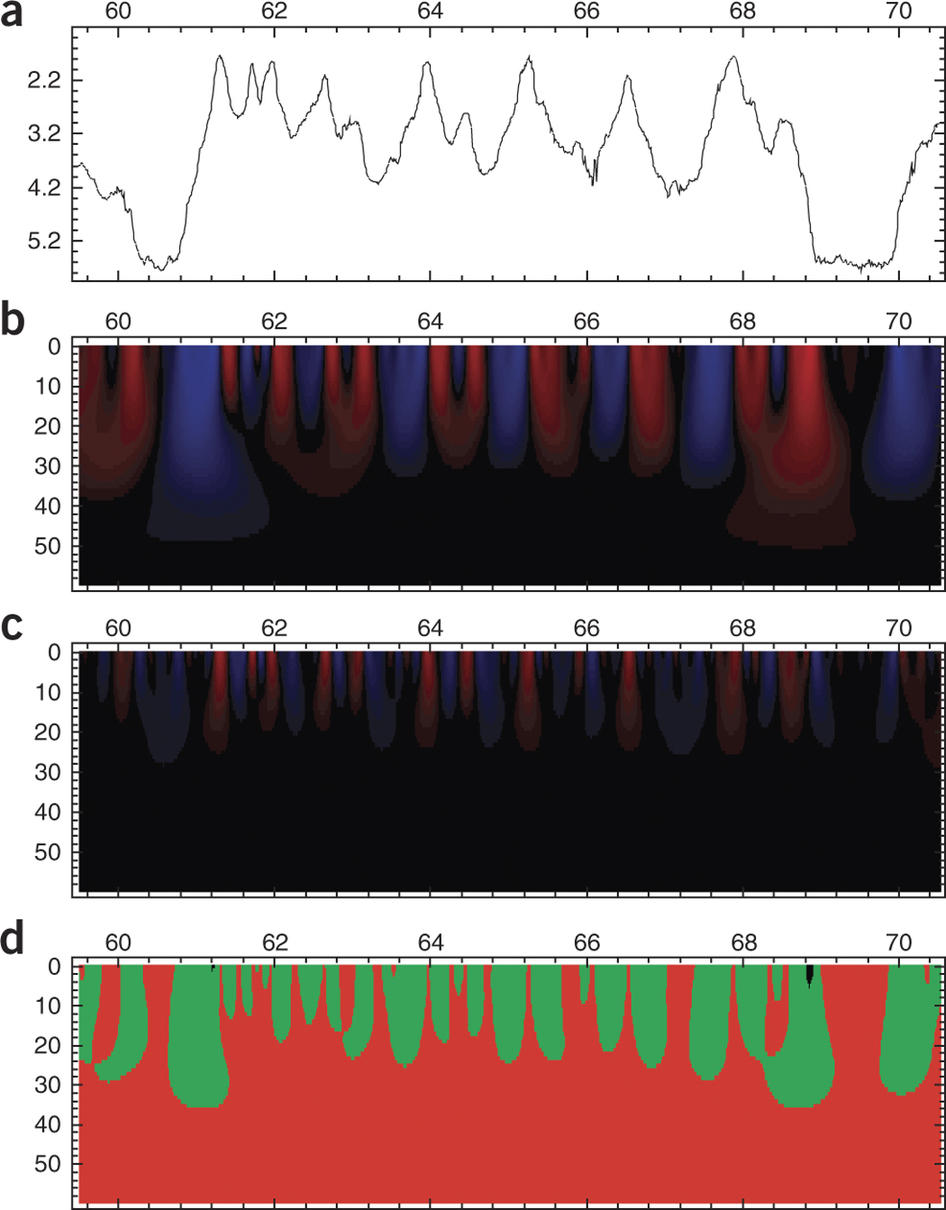
\includegraphics[width=1in]{multiscale_DNA}};
\node[below=0cm of DNA, align=center, text width=1in](DNA_text){DNA replication \\ {\scriptsize Audit {\em et al}, {\em Nature Protocols}, 2013 \par}};

\node[right=of DNA](network_traffic){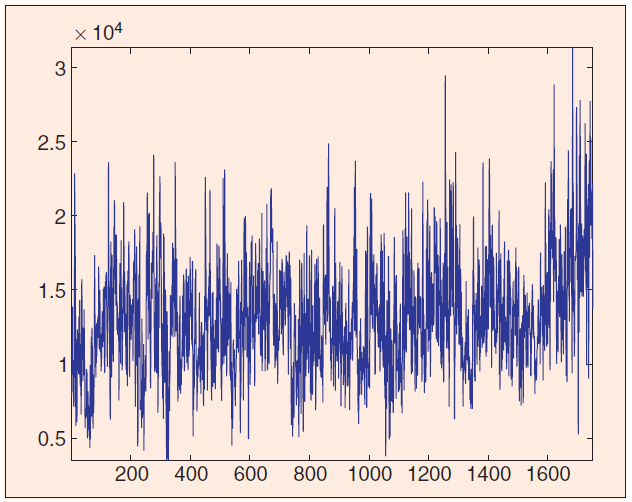
\includegraphics[width=1in]{multiscale_network_traffic}};
\node[below=0cm of network_traffic, align=center, text width=1in](network_traffic_text){Network traffic \\ {\scriptsize Abry {\em et al}, {\em IEEE Signal Processing Magazine}, 2002 \par}};

\end{tikzpicture}


\begin{itemize}
\item Stock market
\item Internet traffic
\item Molecular dynamics
\item Ocean/atmosphere sciences
\item Biology
\end{itemize}

Would like to extract the {\em slow variables} that govern the system dynamics

\end{frame}


\begin{frame}{How to Reduce?}

\begin{block}{Model reduction}

\centering
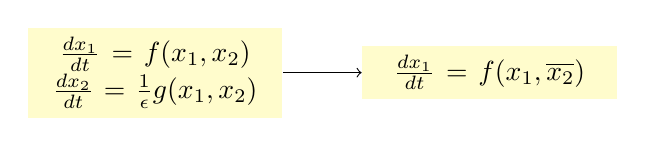
\begin{tikzpicture}
\node[fill=yellow!20, text width=3cm, align=center](a) {$ \frac{dx_1}{dt} = f(x_1,x_2) $ $ \frac{dx_2}{dt} = \frac{1}{\epsilon} g(x_1,x_2)$};
\node[right=of a,fill=yellow!20, text width=3cm, align=center](b) {$ \frac{dx_1}{dt} = f(x_1,\overline{x_2}) $};

\draw[->] (a) -- (b);
\end{tikzpicture}
\end{block}

\begin{block}{Data reduction}

\centering
\begin{tikzpicture}
\node(a) {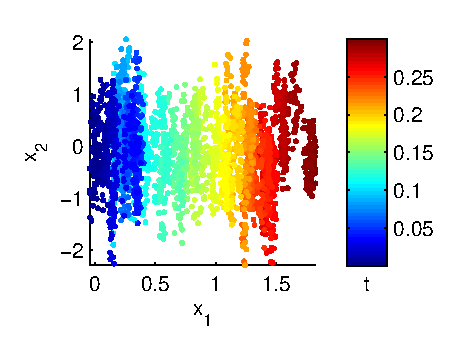
\includegraphics[width=0.35\textwidth]{data_init}};
\node[right=of a](b) {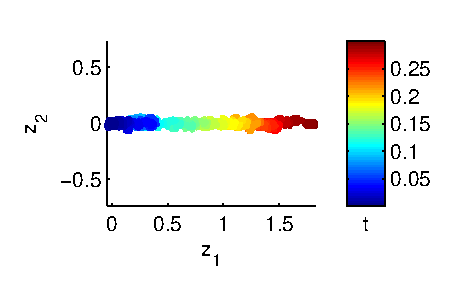
\includegraphics[width=0.35\textwidth]{data_rescaled}};

\draw[->] (a) -- (b);
\end{tikzpicture}

\end{block}

We will focus on the second case: {\bf data reduction}
\end{frame}

%\begin{frame}{Outline}
%
%\tableofcontents
%%\begin{itemize}
%%\item Multiscale SDE framework
%%\item Data reduction (diffusion maps)
%%\item Mahalnobis distance to capture relevant timescales
%%\item Examples
%%\item Conclusion/applications/future work
%%\end{itemize}
%
%\end{frame}


\section{Multiscale SDEs}

\begin{frame}{Assumed Model for Multiscale Data}


\begin{tikzpicture}

\node[fill=orange!20](a) {$\begin{aligned}
dx_i(t) &= a_i(\vec{x}(t)) dt + dW_i(t), & \: 1 \le i \le m \\
dx_i(t) &= \frac{a_i(\vec{x}(t))}{\epsilon} dt + \frac{1}{\sqrt{\epsilon}} dW_i(t) , & \: m+1 \le i \le n
\end{aligned}$};

\node[below=0.5cm of a, text width=0.5\textwidth,fill=yellow!20](text1){small parameter $\epsilon$ creates separation of timescales};
\node[above right=0cm and 0cm of a, text width=0.2\textwidth,fill=yellow!20](text2){$m$ slow variables};

\node[below right=0cm and 0cm of a, text width=0.2\textwidth,fill=yellow!20](text3){$n-m$ fast~variables};


\draw[<-] (-2,-0.75)--(text1);
\draw[<-] (0,-0.75)--(text1);

\draw[<-] (4,0.8)--(text2.west);
\draw[<-] (4,-0.75)--(text3.west);


\end{tikzpicture}

Under some mild conditions, we can write a {\em reduced} SDE 

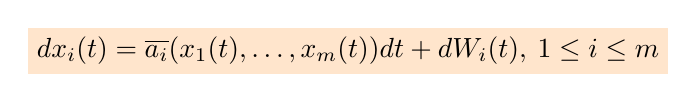
\begin{tikzpicture}

\node[fill=orange!20](a) {$dx_i(t) = \overline{a_i}(x_1(t), \dots, x_m(t)) dt + dW_i(t), \: 1 \le i \le m $};

\end{tikzpicture}

We will discuss how we can extract a parameterization of $x_1, \dots, x_m$ from {\em data}

\end{frame}

\section{Data Reduction}

\begin{frame}{Data Reduction in General}

\begin{tikzpicture}

\node(a){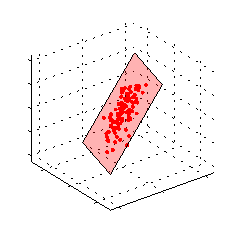
\includegraphics{PCA_3D}};
\node(texta)[below=0cm of a, text width=4.5cm, align=center] {High dimensional data on low-dimensional structure};
\node[right=2cm of a](b){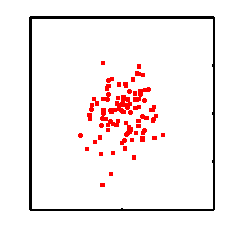
\includegraphics{PCA_2D}};
\node(texba)[below=0cm of b, text width=4cm, align=center] {Want to reduce dimensionality};
\draw[->] (a) -- (b);
\end{tikzpicture}

Most common technique: Principal Component Analysis

\newfootnote{Shlens, ``A Tutorial on Principal Component Analysys}
\end{frame}

\begin{frame}{Diffusion Maps for Nonlinear Data Reduction}
    
    \centering
    \begin{tikzpicture}
        \node (fig1) {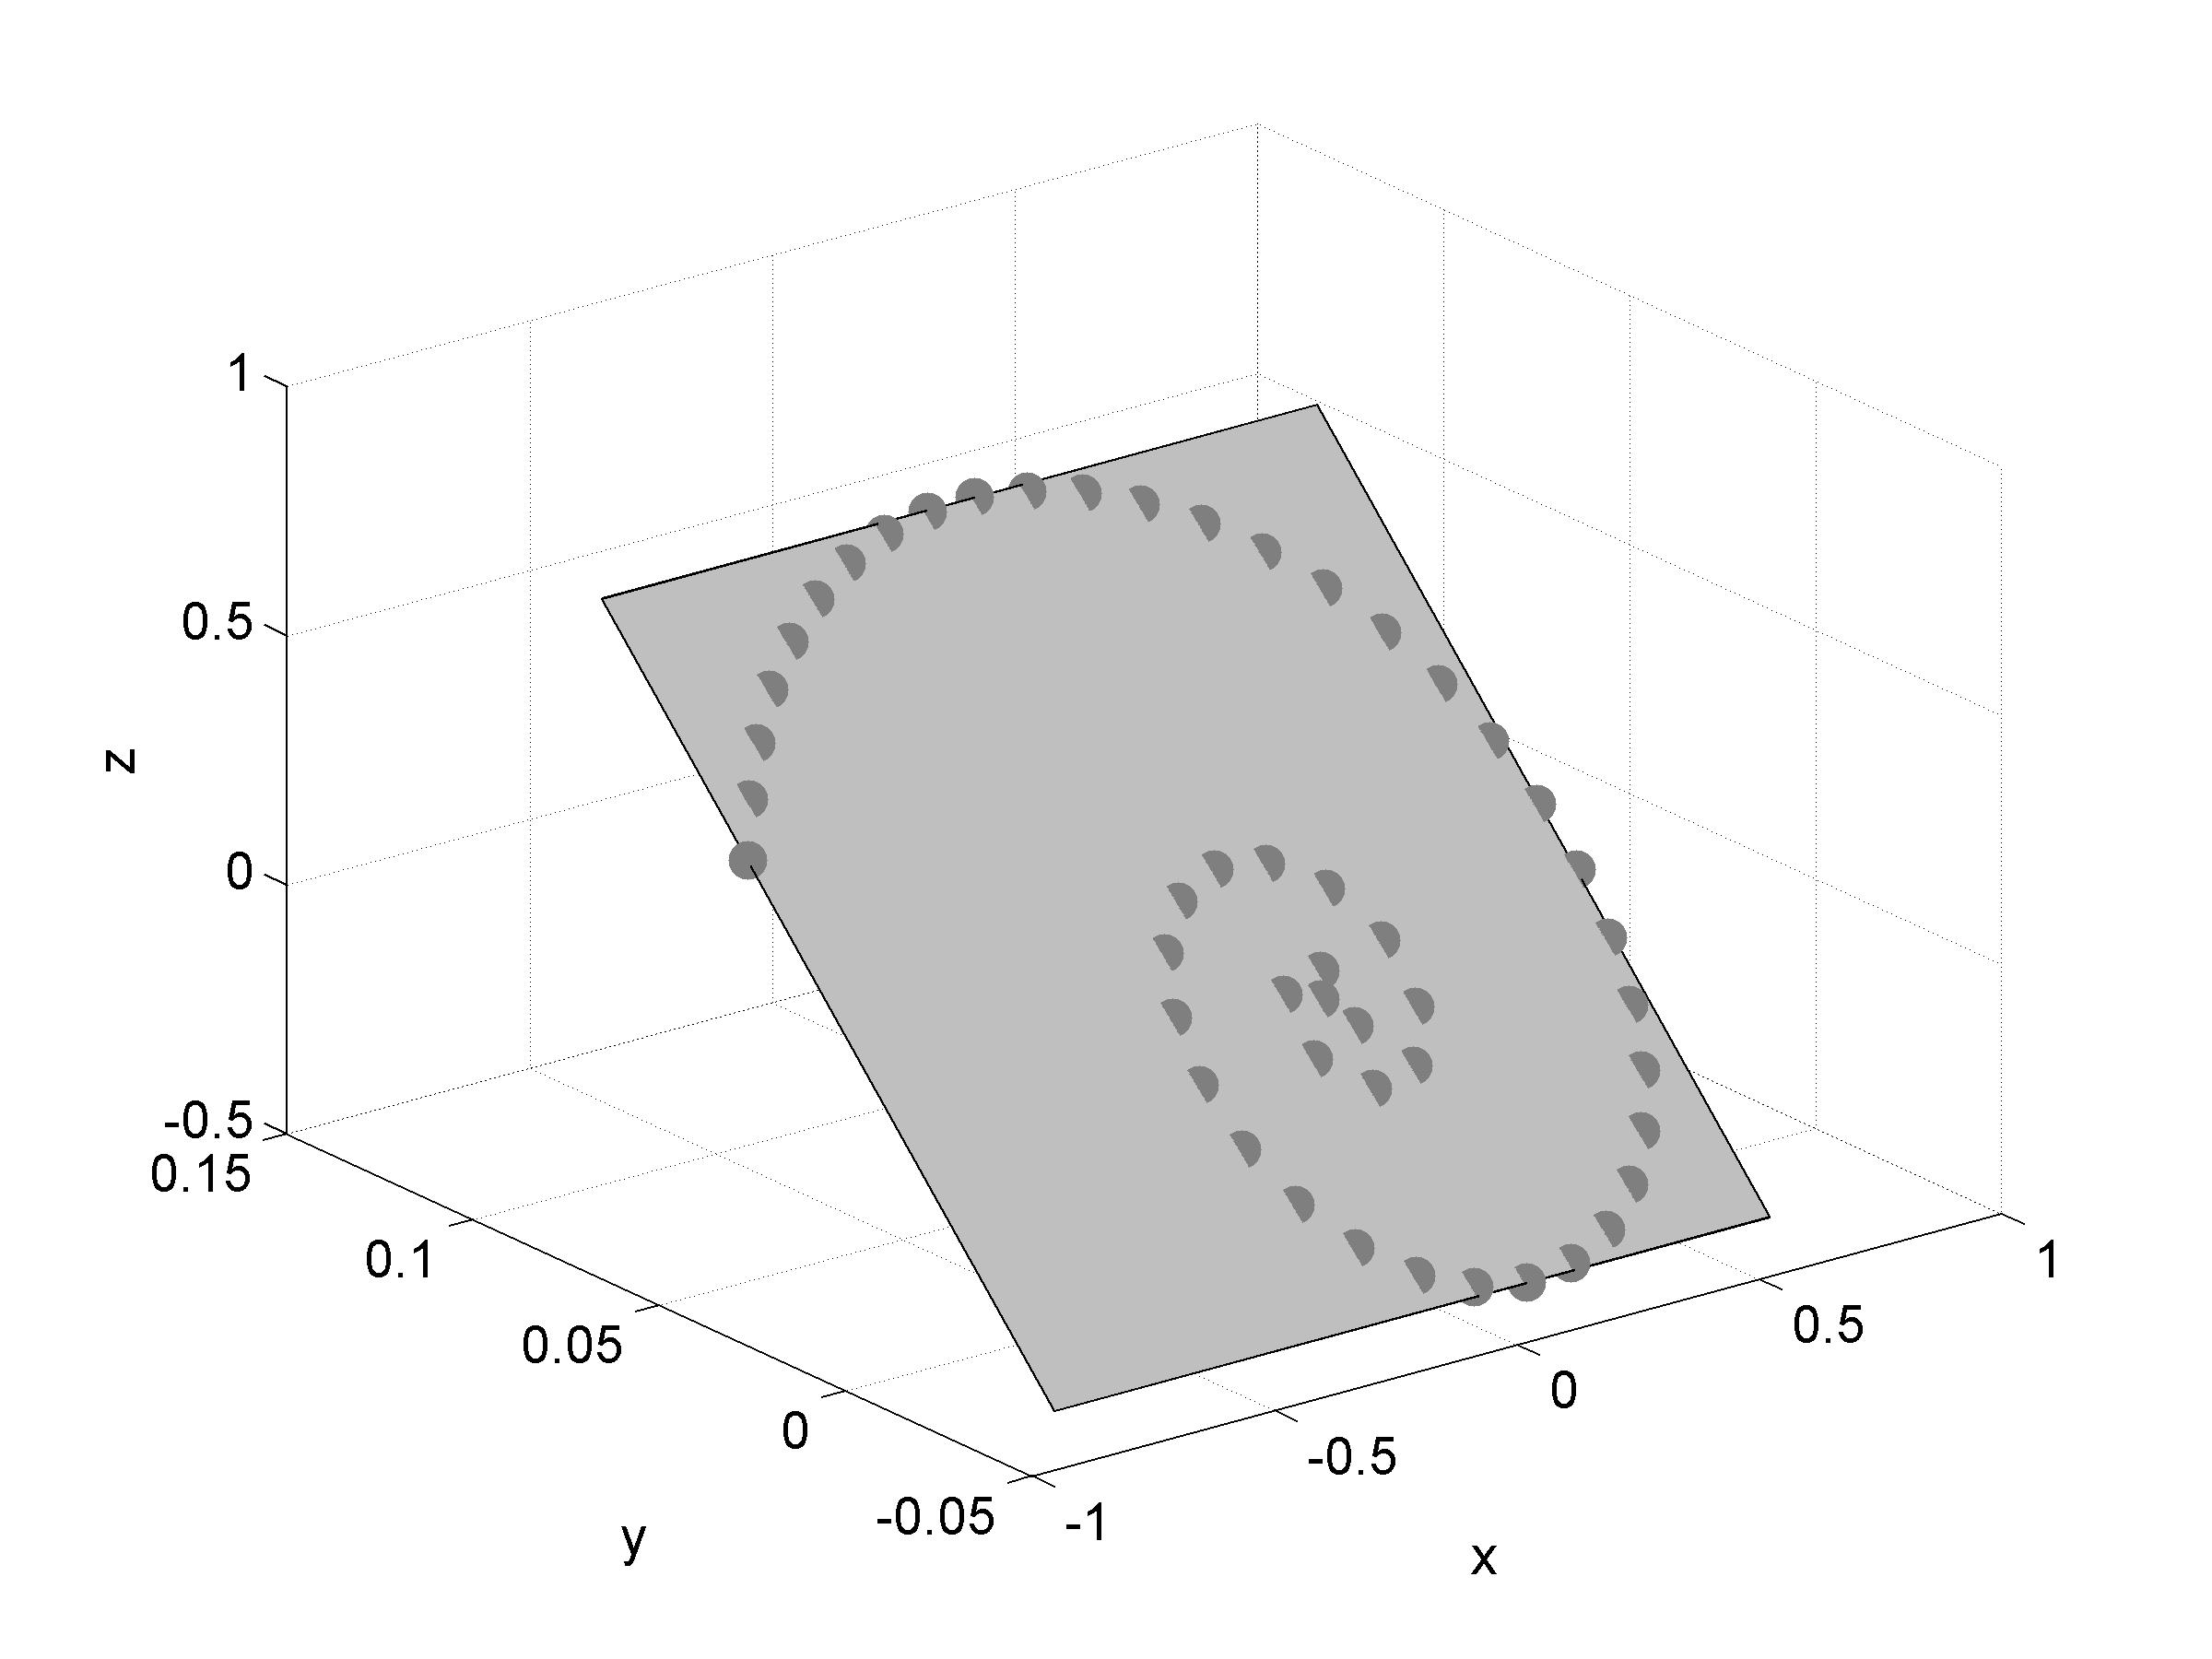
\includegraphics[width=0.4\textwidth]{dmaps_spiral_black_plane_large.jpg}};
        \draw[red,->] (-0.15,-1.2) -- (0.9, -0.9);
        \draw[red,->] (-0.15,-1.2) -- (-1, 0.4);
        \node[right of=fig1, node distance=0.5\textwidth] (fig2) {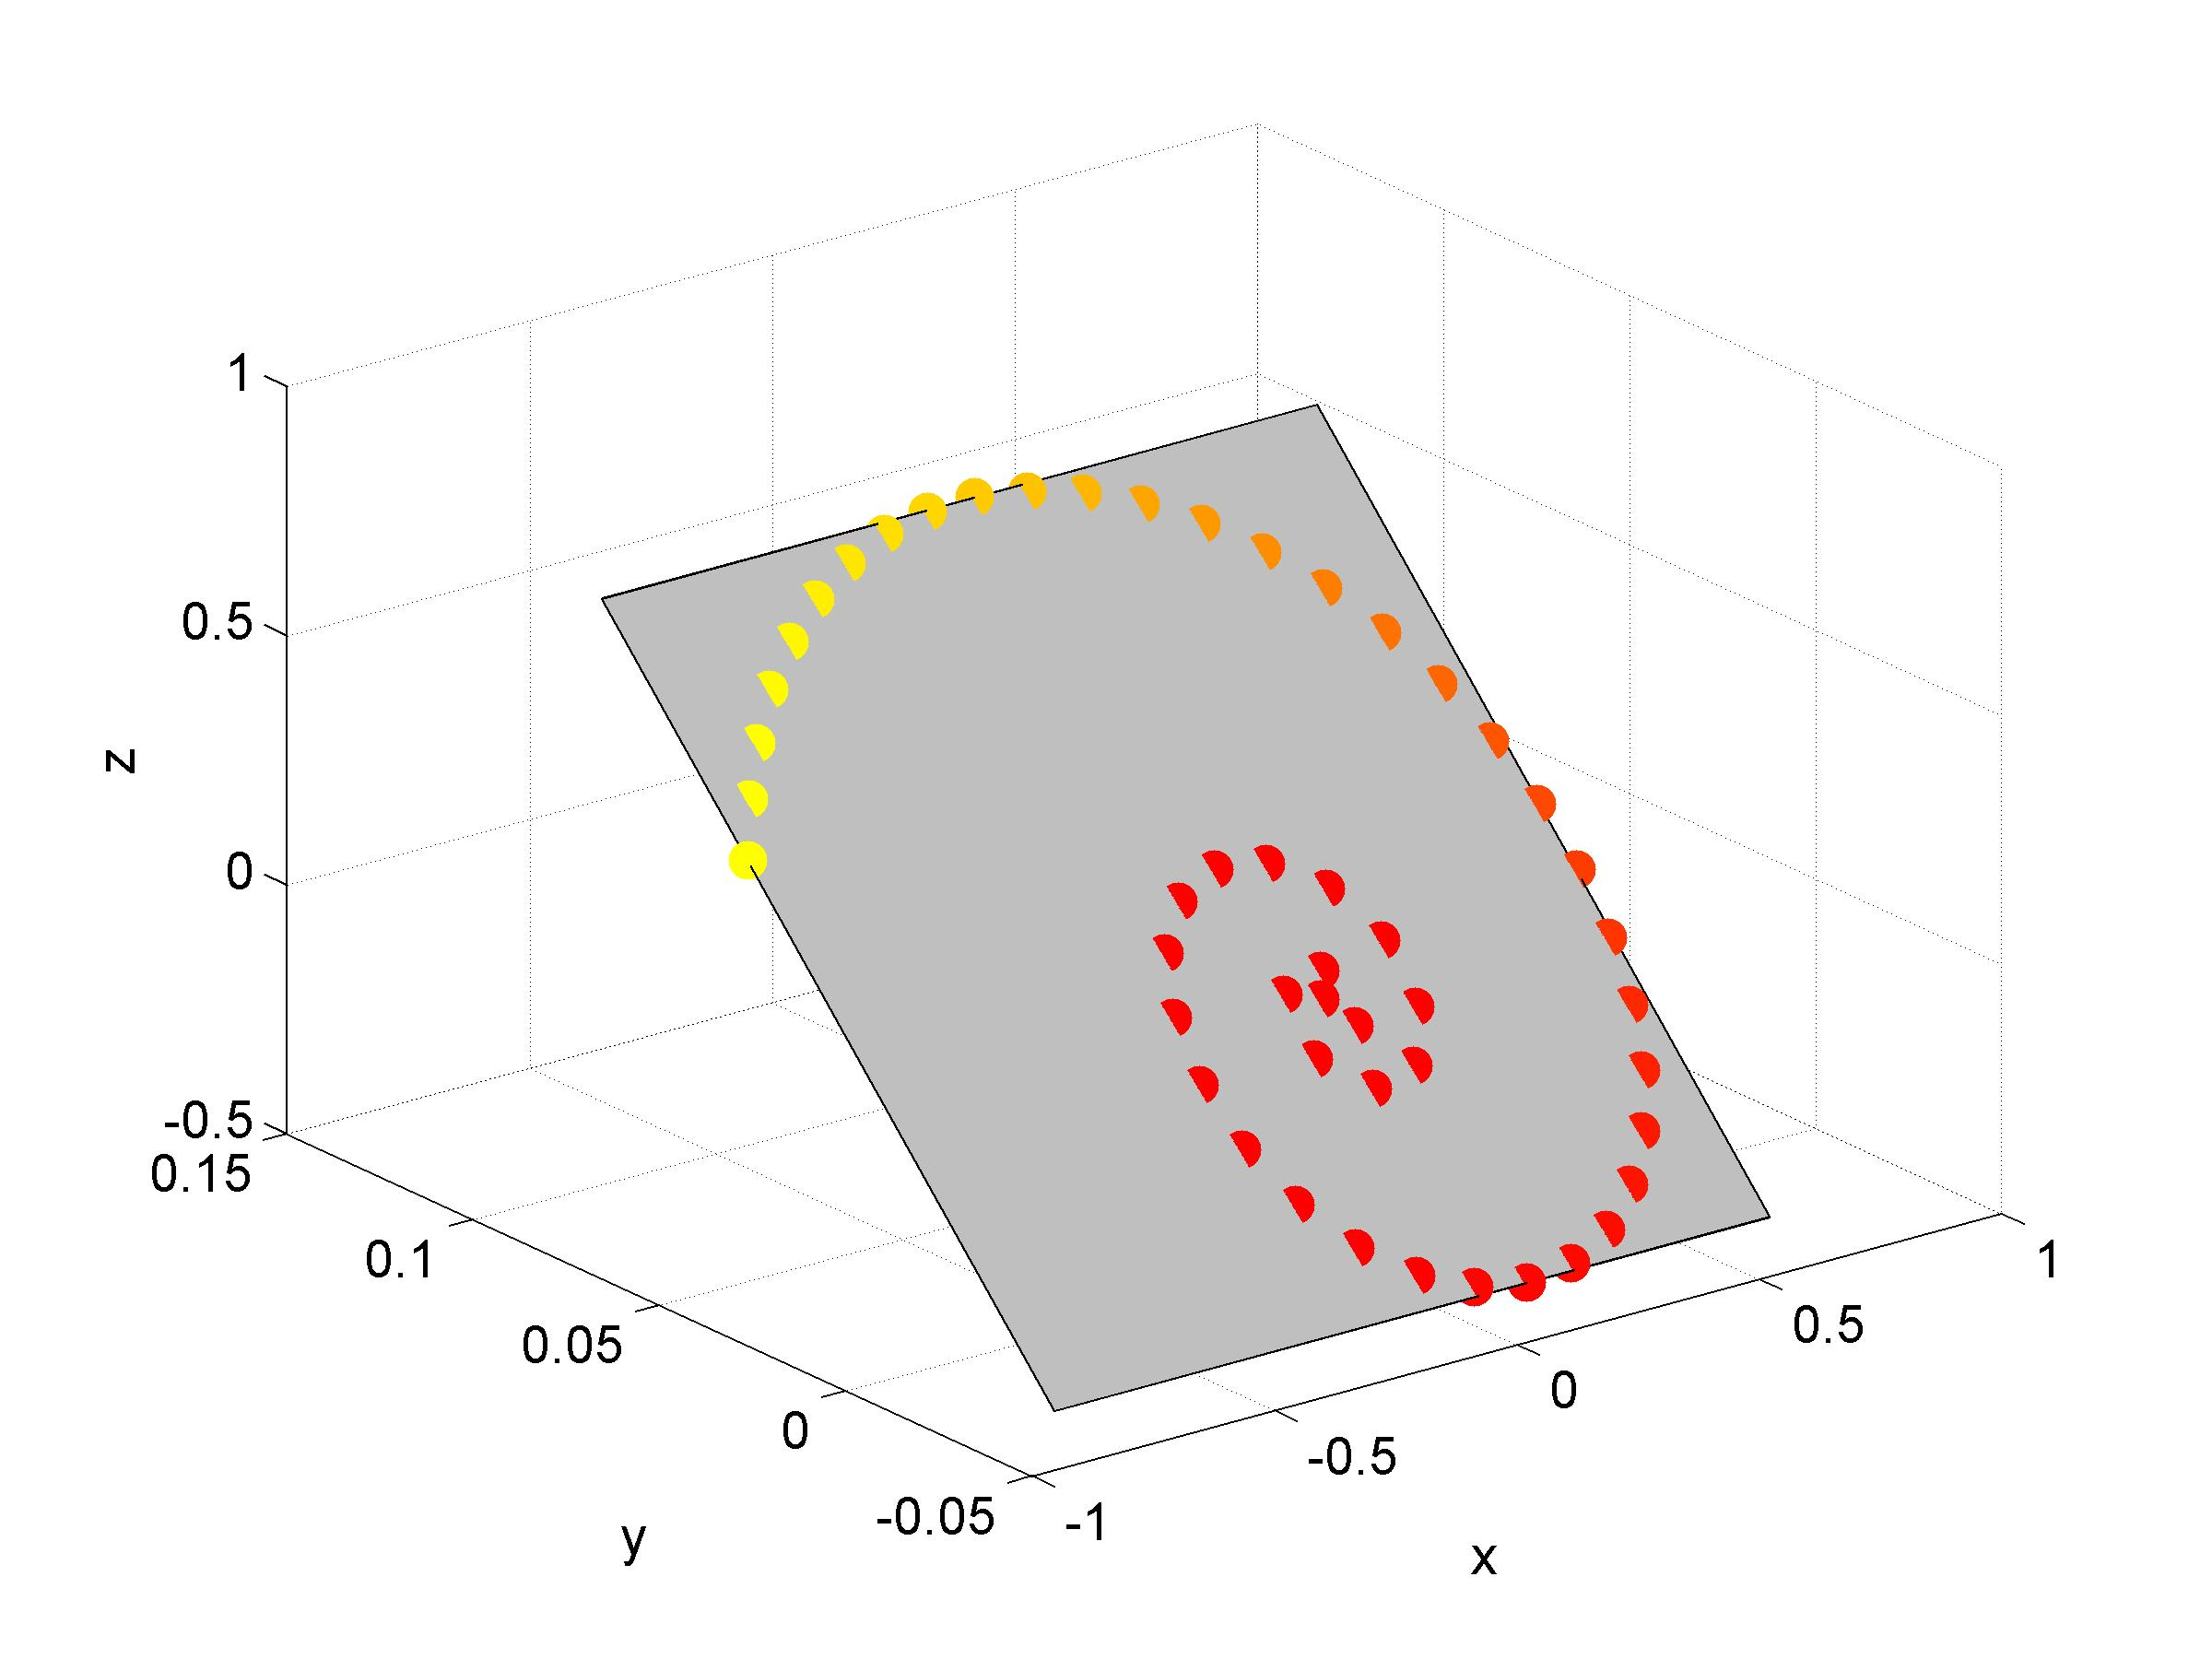
\includegraphics[width=0.4\textwidth]{dmaps_spiral_color_plane_large.jpg}};
        \draw [->] (fig1.east) -- (fig2.west);
        
        \node[below=0cm of fig1, text width=0.3\textwidth, align=center]{Data on a spiral \\ {\scriptsize PCA will find the two-dimensional plane \par}};
        
        \node[below=0cm of fig2, text width=0.3\textwidth, align=center]{Data colored by first diffusion maps coordinate};
        
    \end{tikzpicture}

	\newfootnote{Coifman {\em et al}, PNAS, 2005.}

\end{frame}

\begin{frame}{Eigenfunctions to Parameterize a Manifold}

    %\vspace{0.15in}
    {\scriptsize
    \begin{minipage}[t]{0.3\textwidth}
        \centering
        Consider a manifold\\
        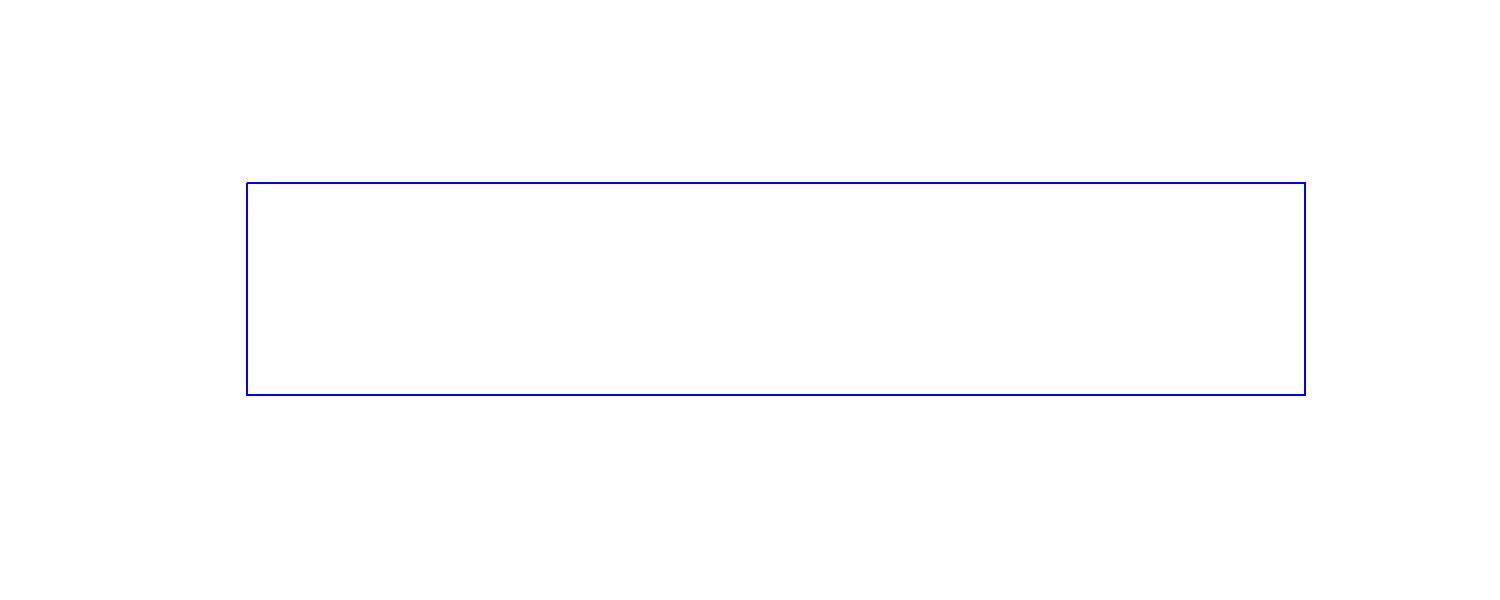
\includegraphics[width=\textwidth]{rect.jpg}\\


    \end{minipage}
    \begin{minipage}[t]{0.35\textwidth}
        \centering
        We want a ``good'' parametrization of~the manifold\\
        \vspace{0.1in}
        \animategraphics[width=\textwidth]{1}{rect_efunc}{1}{6}\\
        \vspace{-0.03in}
        These parameterizations are the~eigenfunctions of $\nabla^2 \phi$\\
    \end{minipage}
    \begin{minipage}[t]{0.3\textwidth}
        \centering
        Instead, we have data {\em sampled} from the manifold and want to~obtain a parameterization\\
        \vspace{0.1in}
        \animategraphics[width=\textwidth]{1}{rect_evec}{1}{6}\\
        \vspace{0.1in}
        We therefore {\em approximate} the~Laplacian on the data
    \end{minipage}
    \par}

    \vspace{0.1in}

    \centering
    {\small We obtain a similar parametrization for a curved manifold \par}
    \vspace{0.05in}
    
\includegraphics[width=0.18\textwidth]{circle.jpg}
    \hspace{0.03\textwidth}
    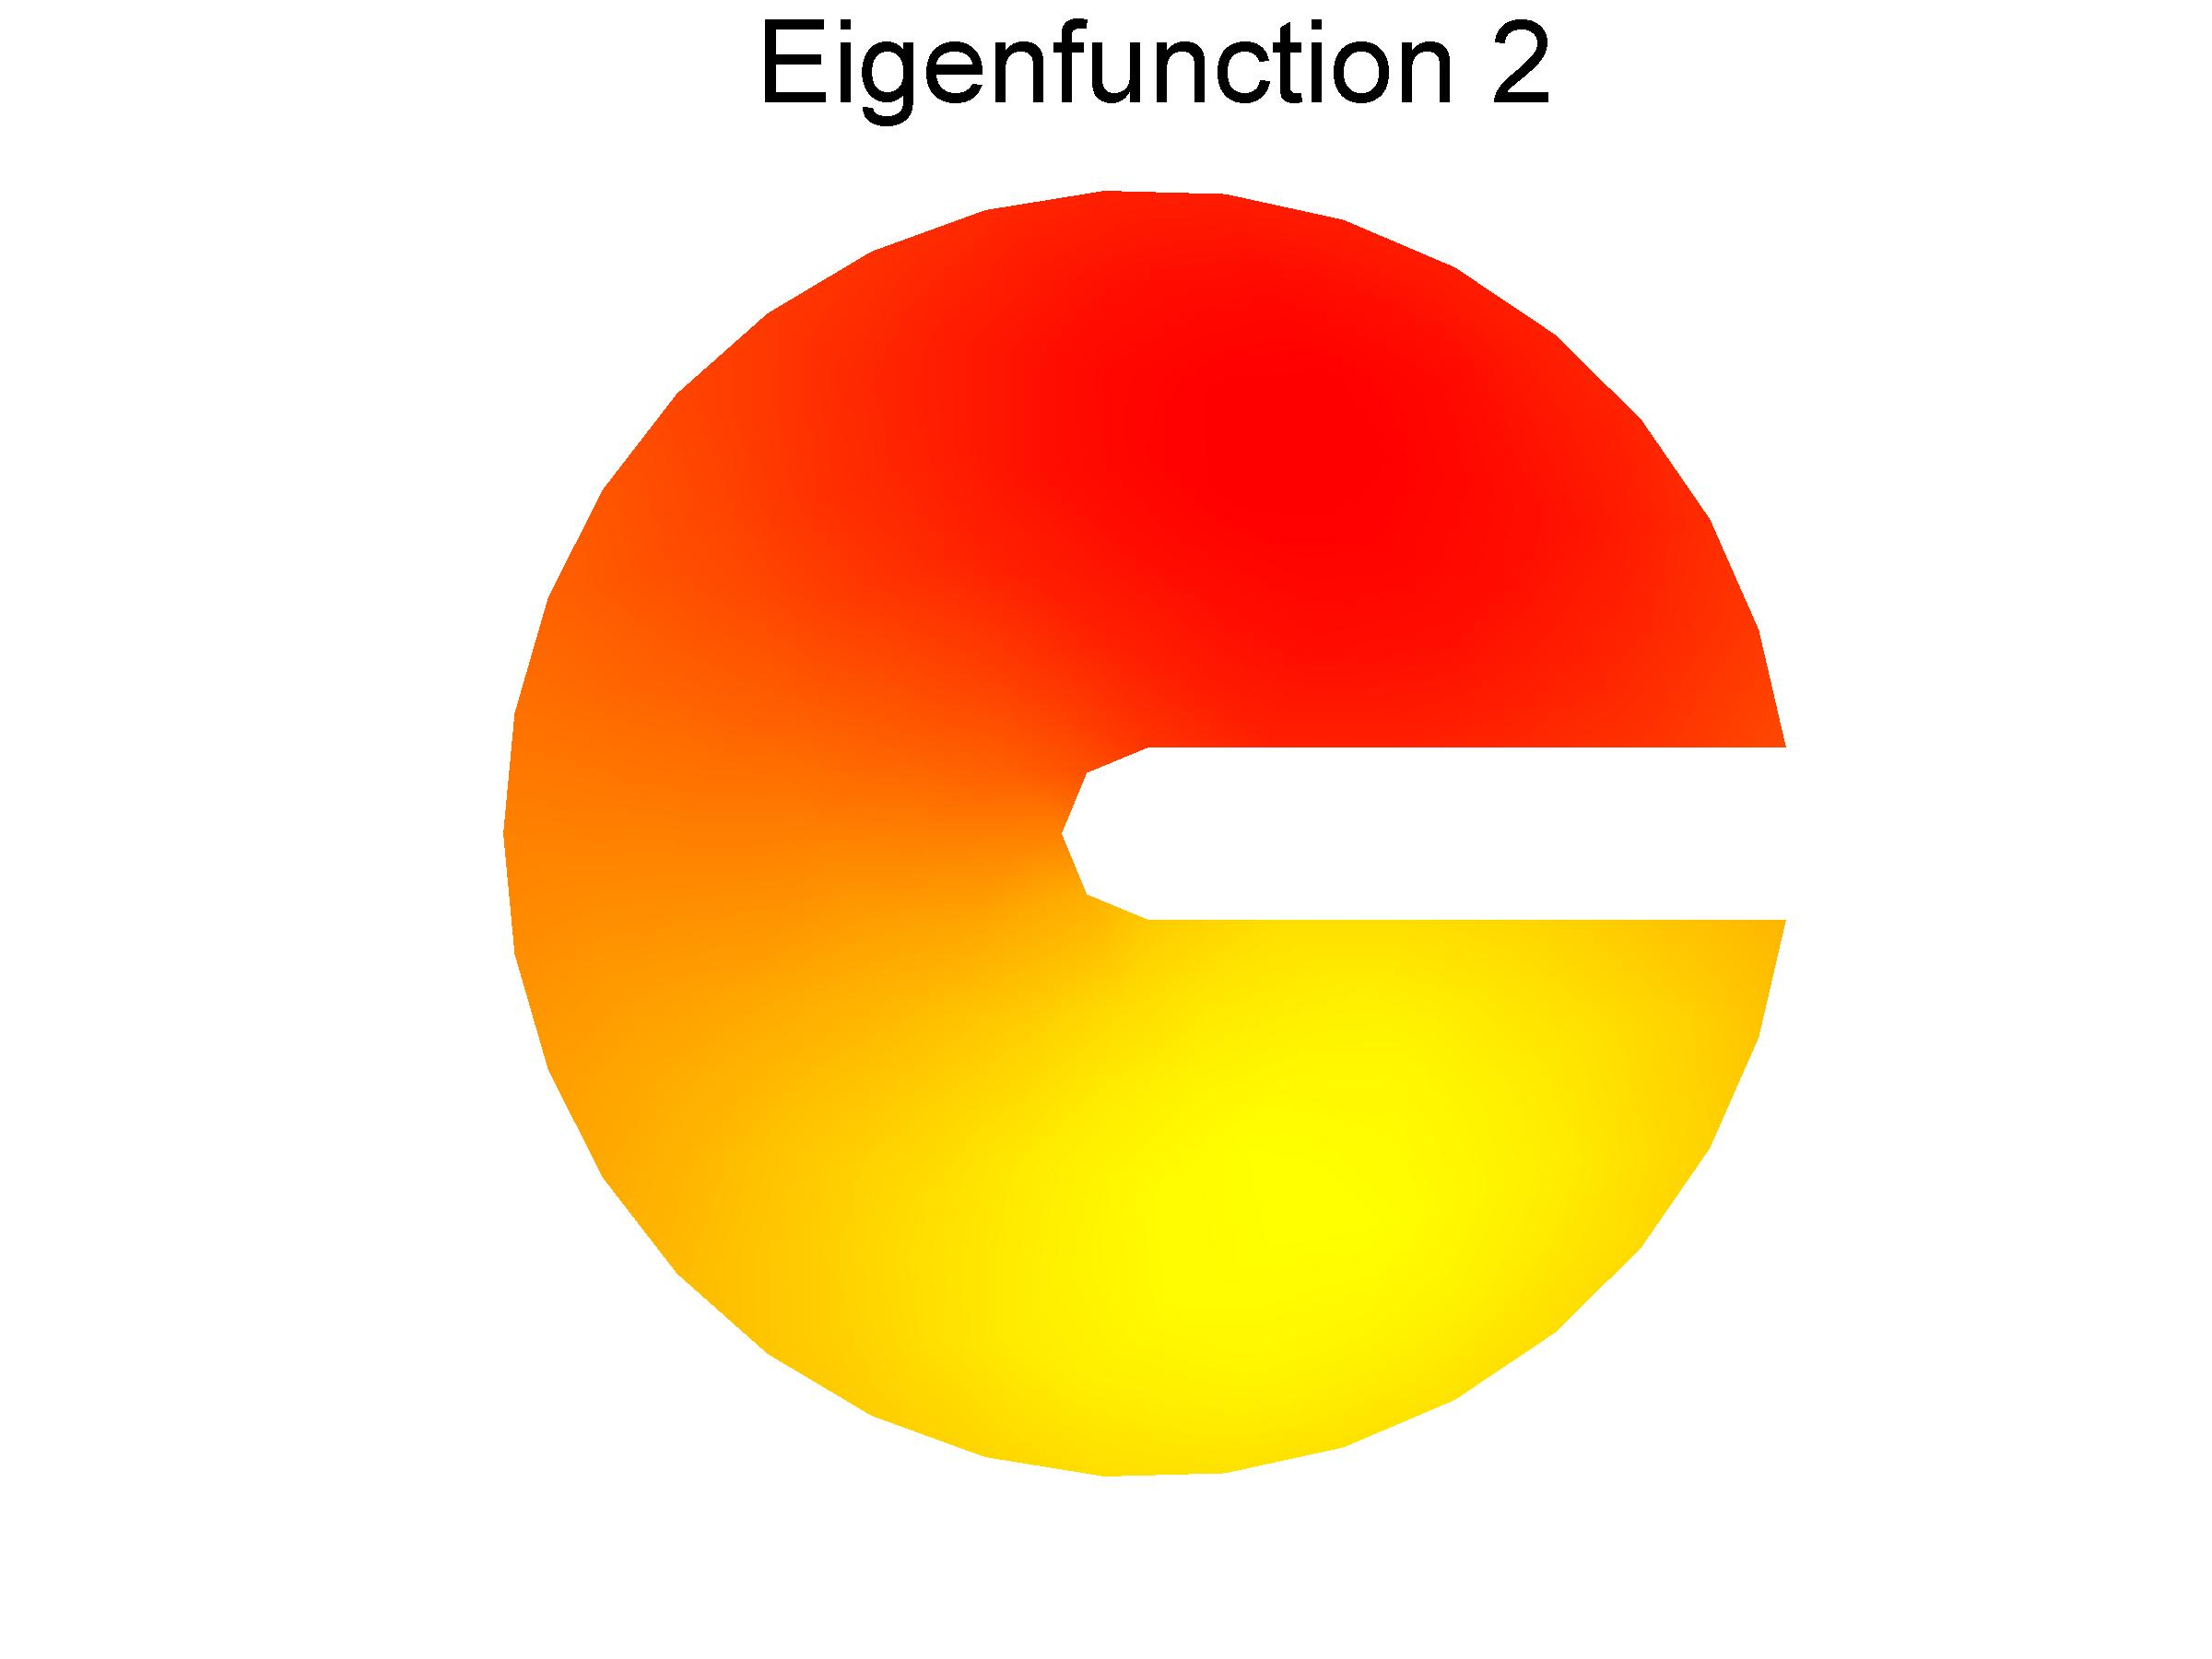
\includegraphics[width=0.18\textwidth]{circle_efunc1.jpg}
    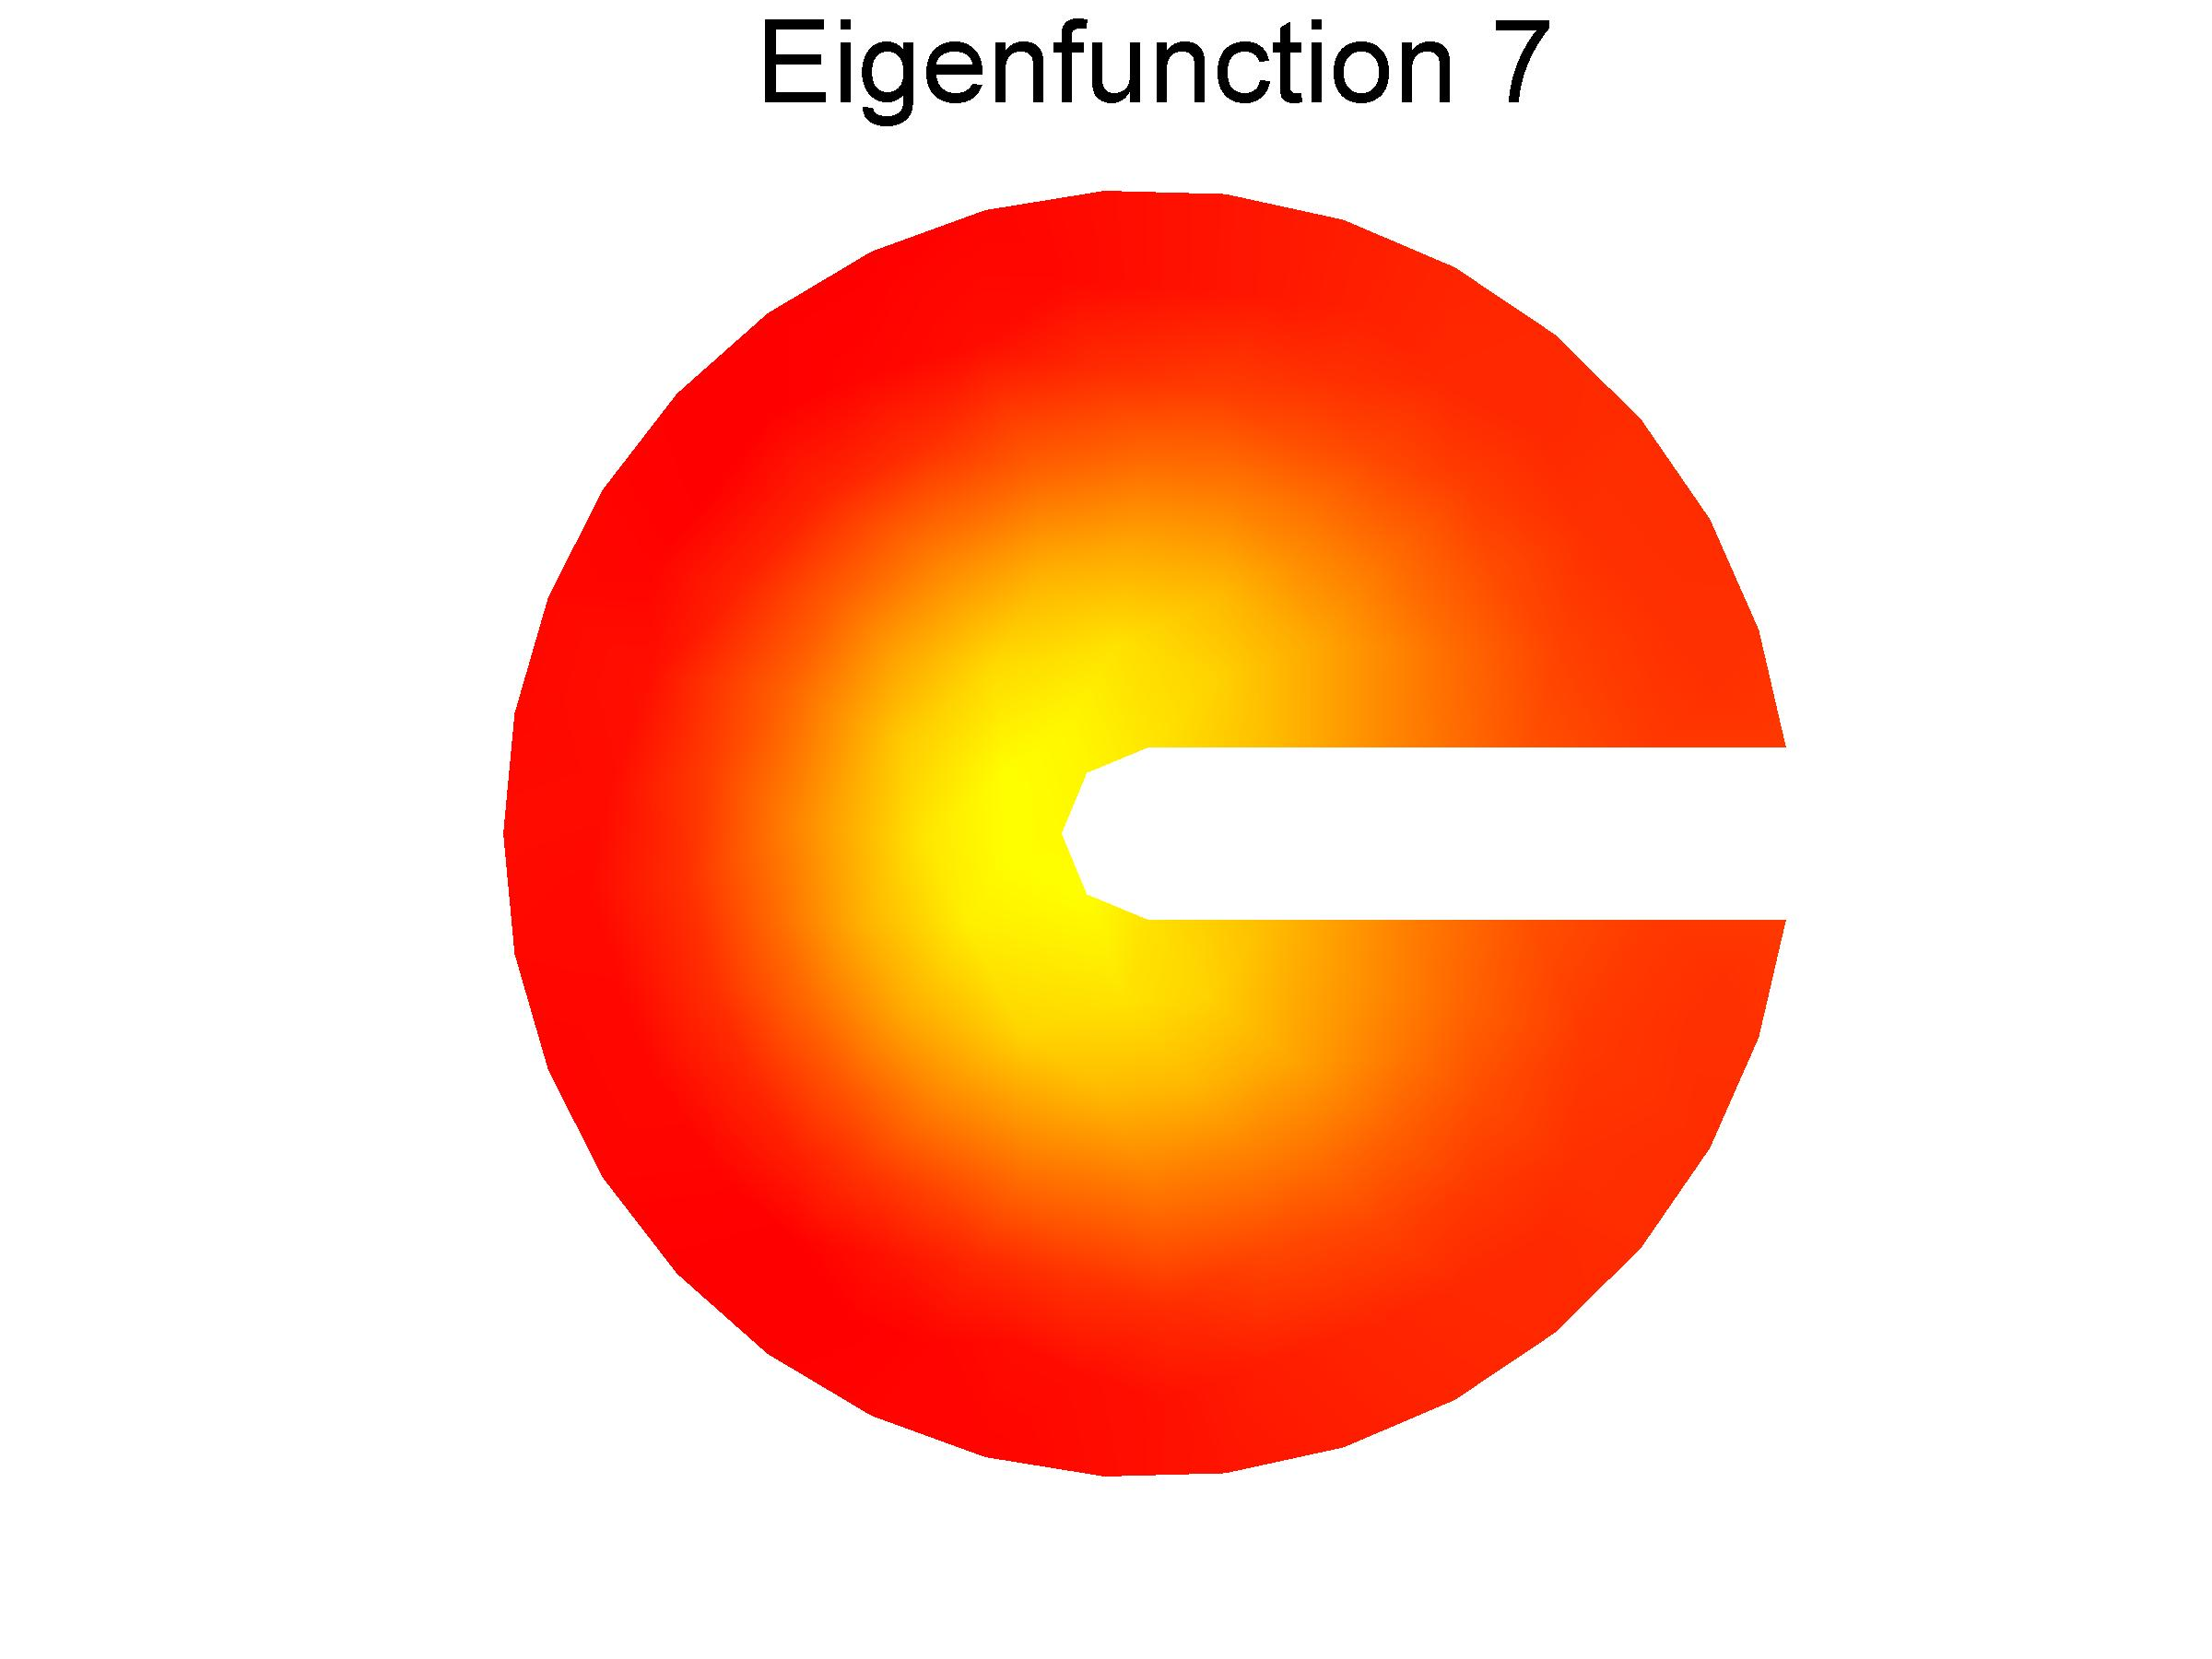
\includegraphics[width=0.18\textwidth]{circle_efunc6.jpg}
    \hspace{0.03\textwidth}
    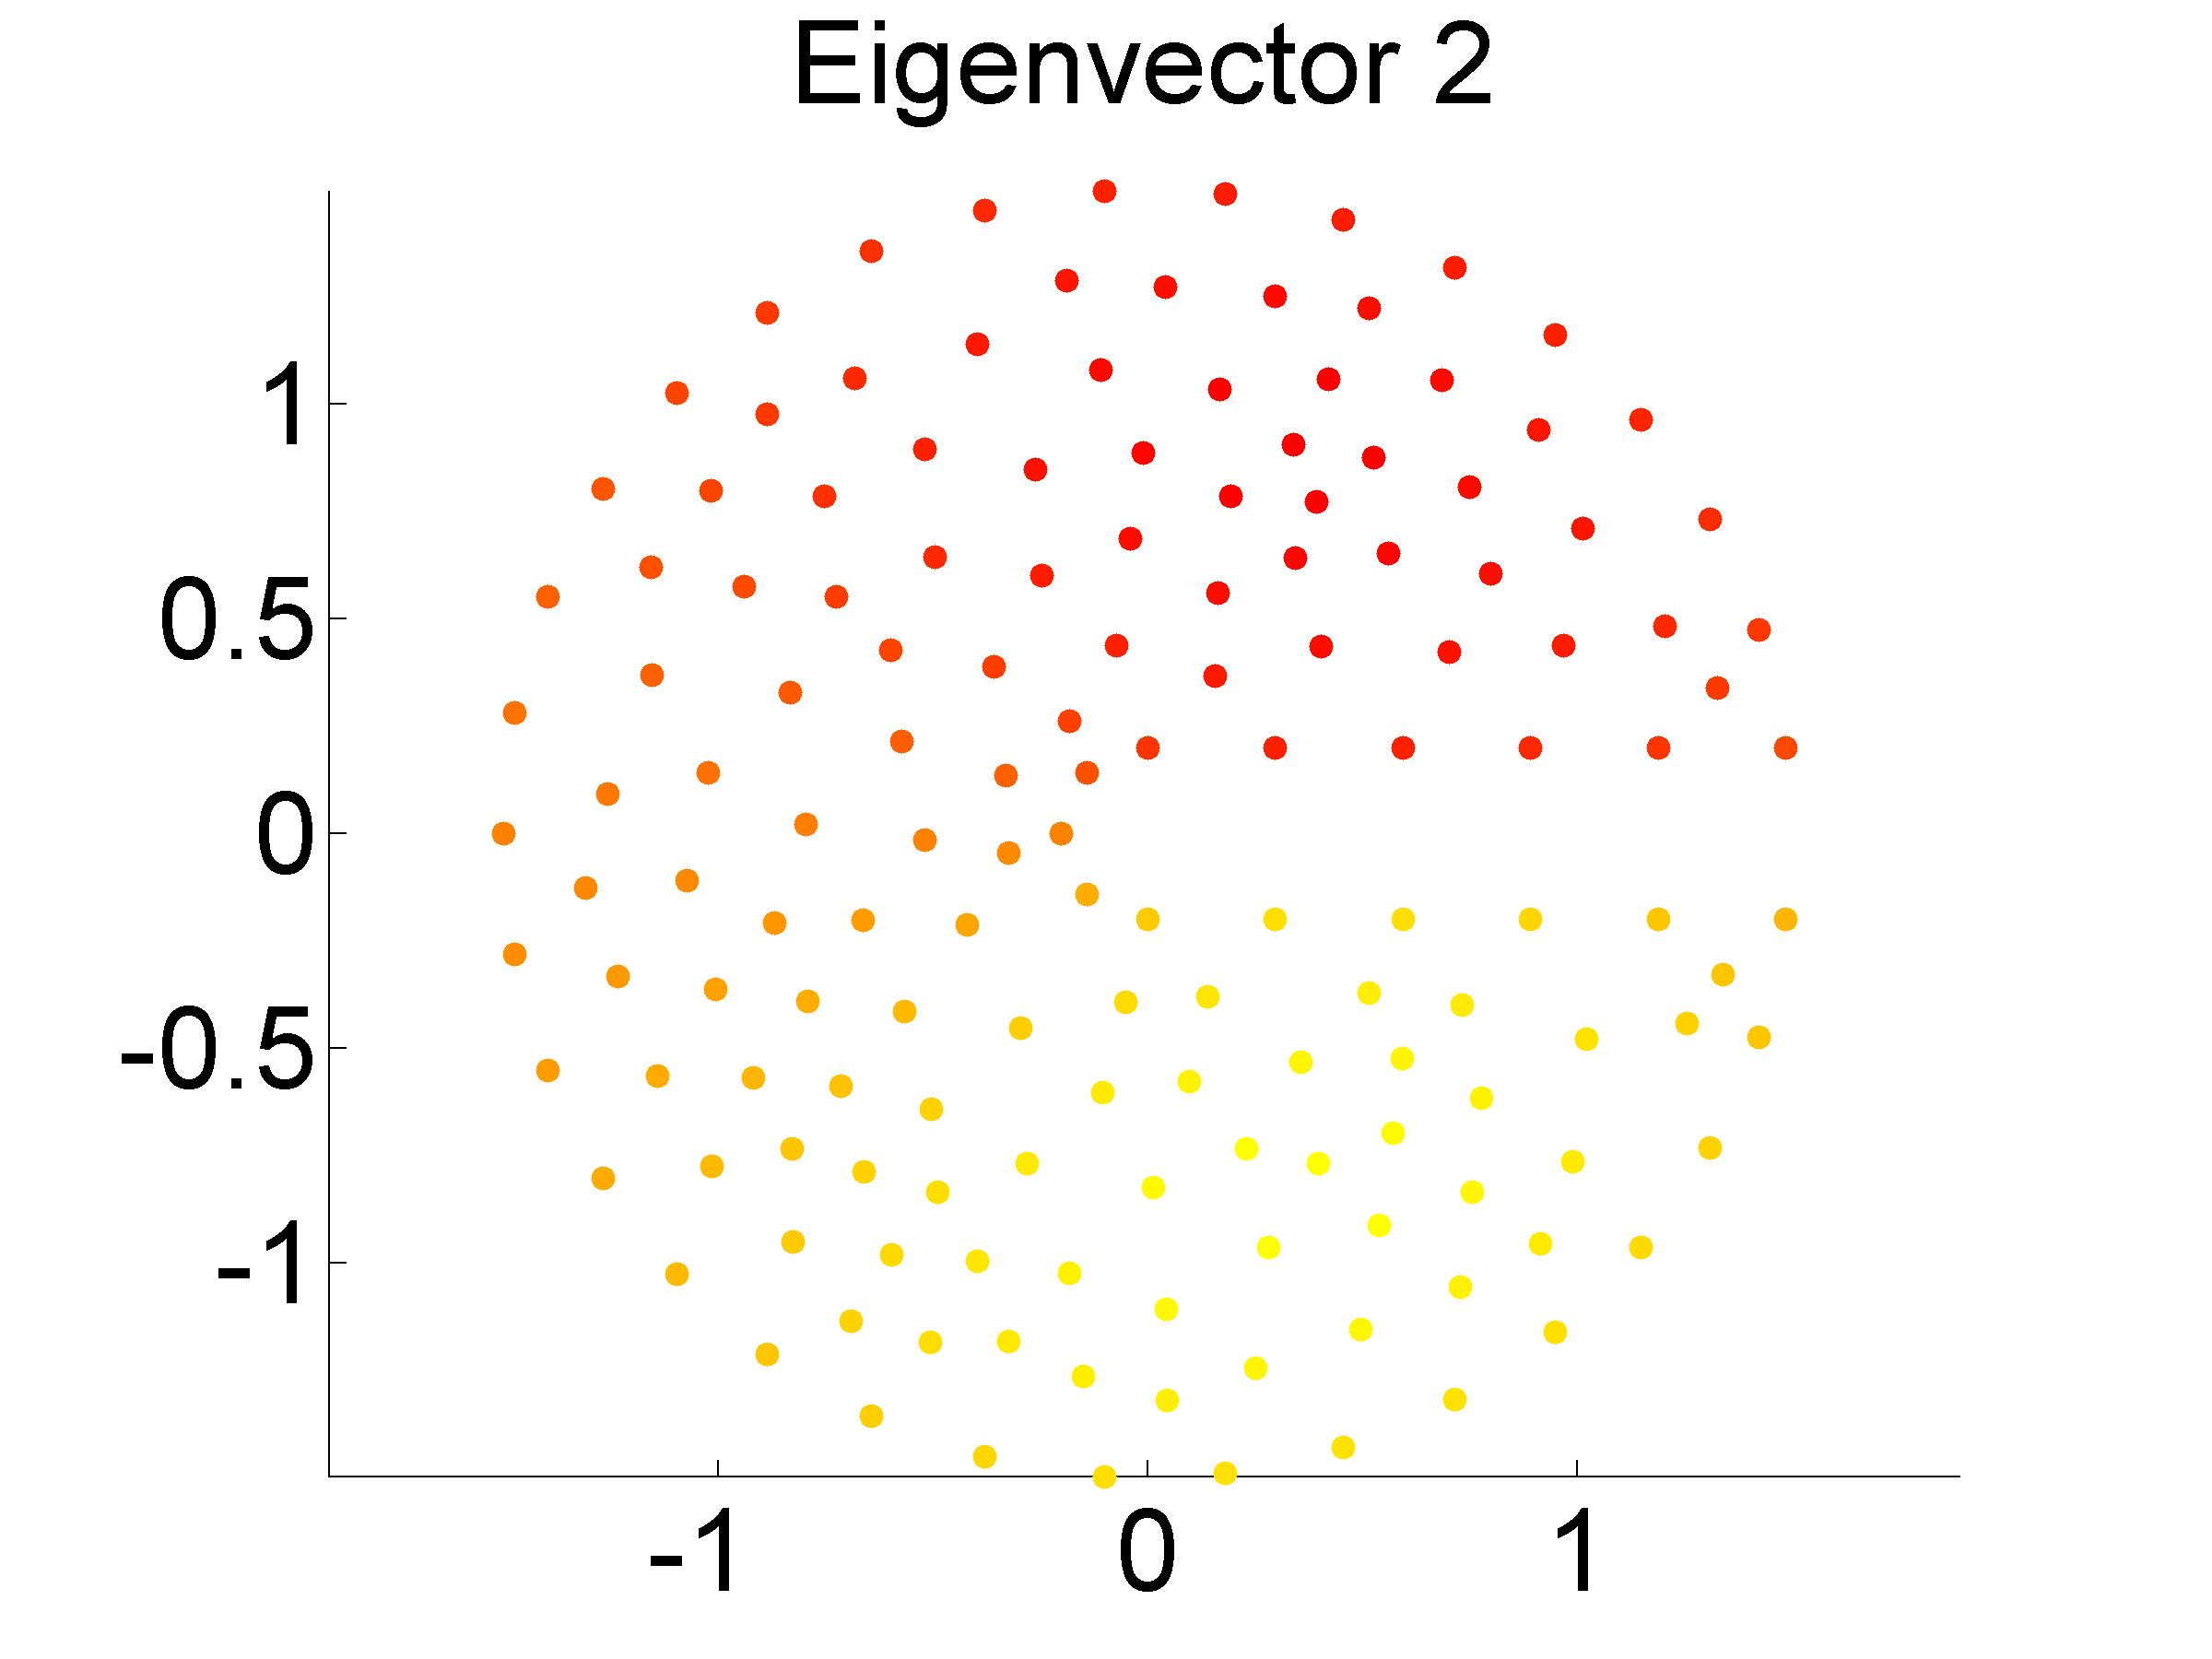
\includegraphics[width=0.18\textwidth]{circle_evec1.jpg}
    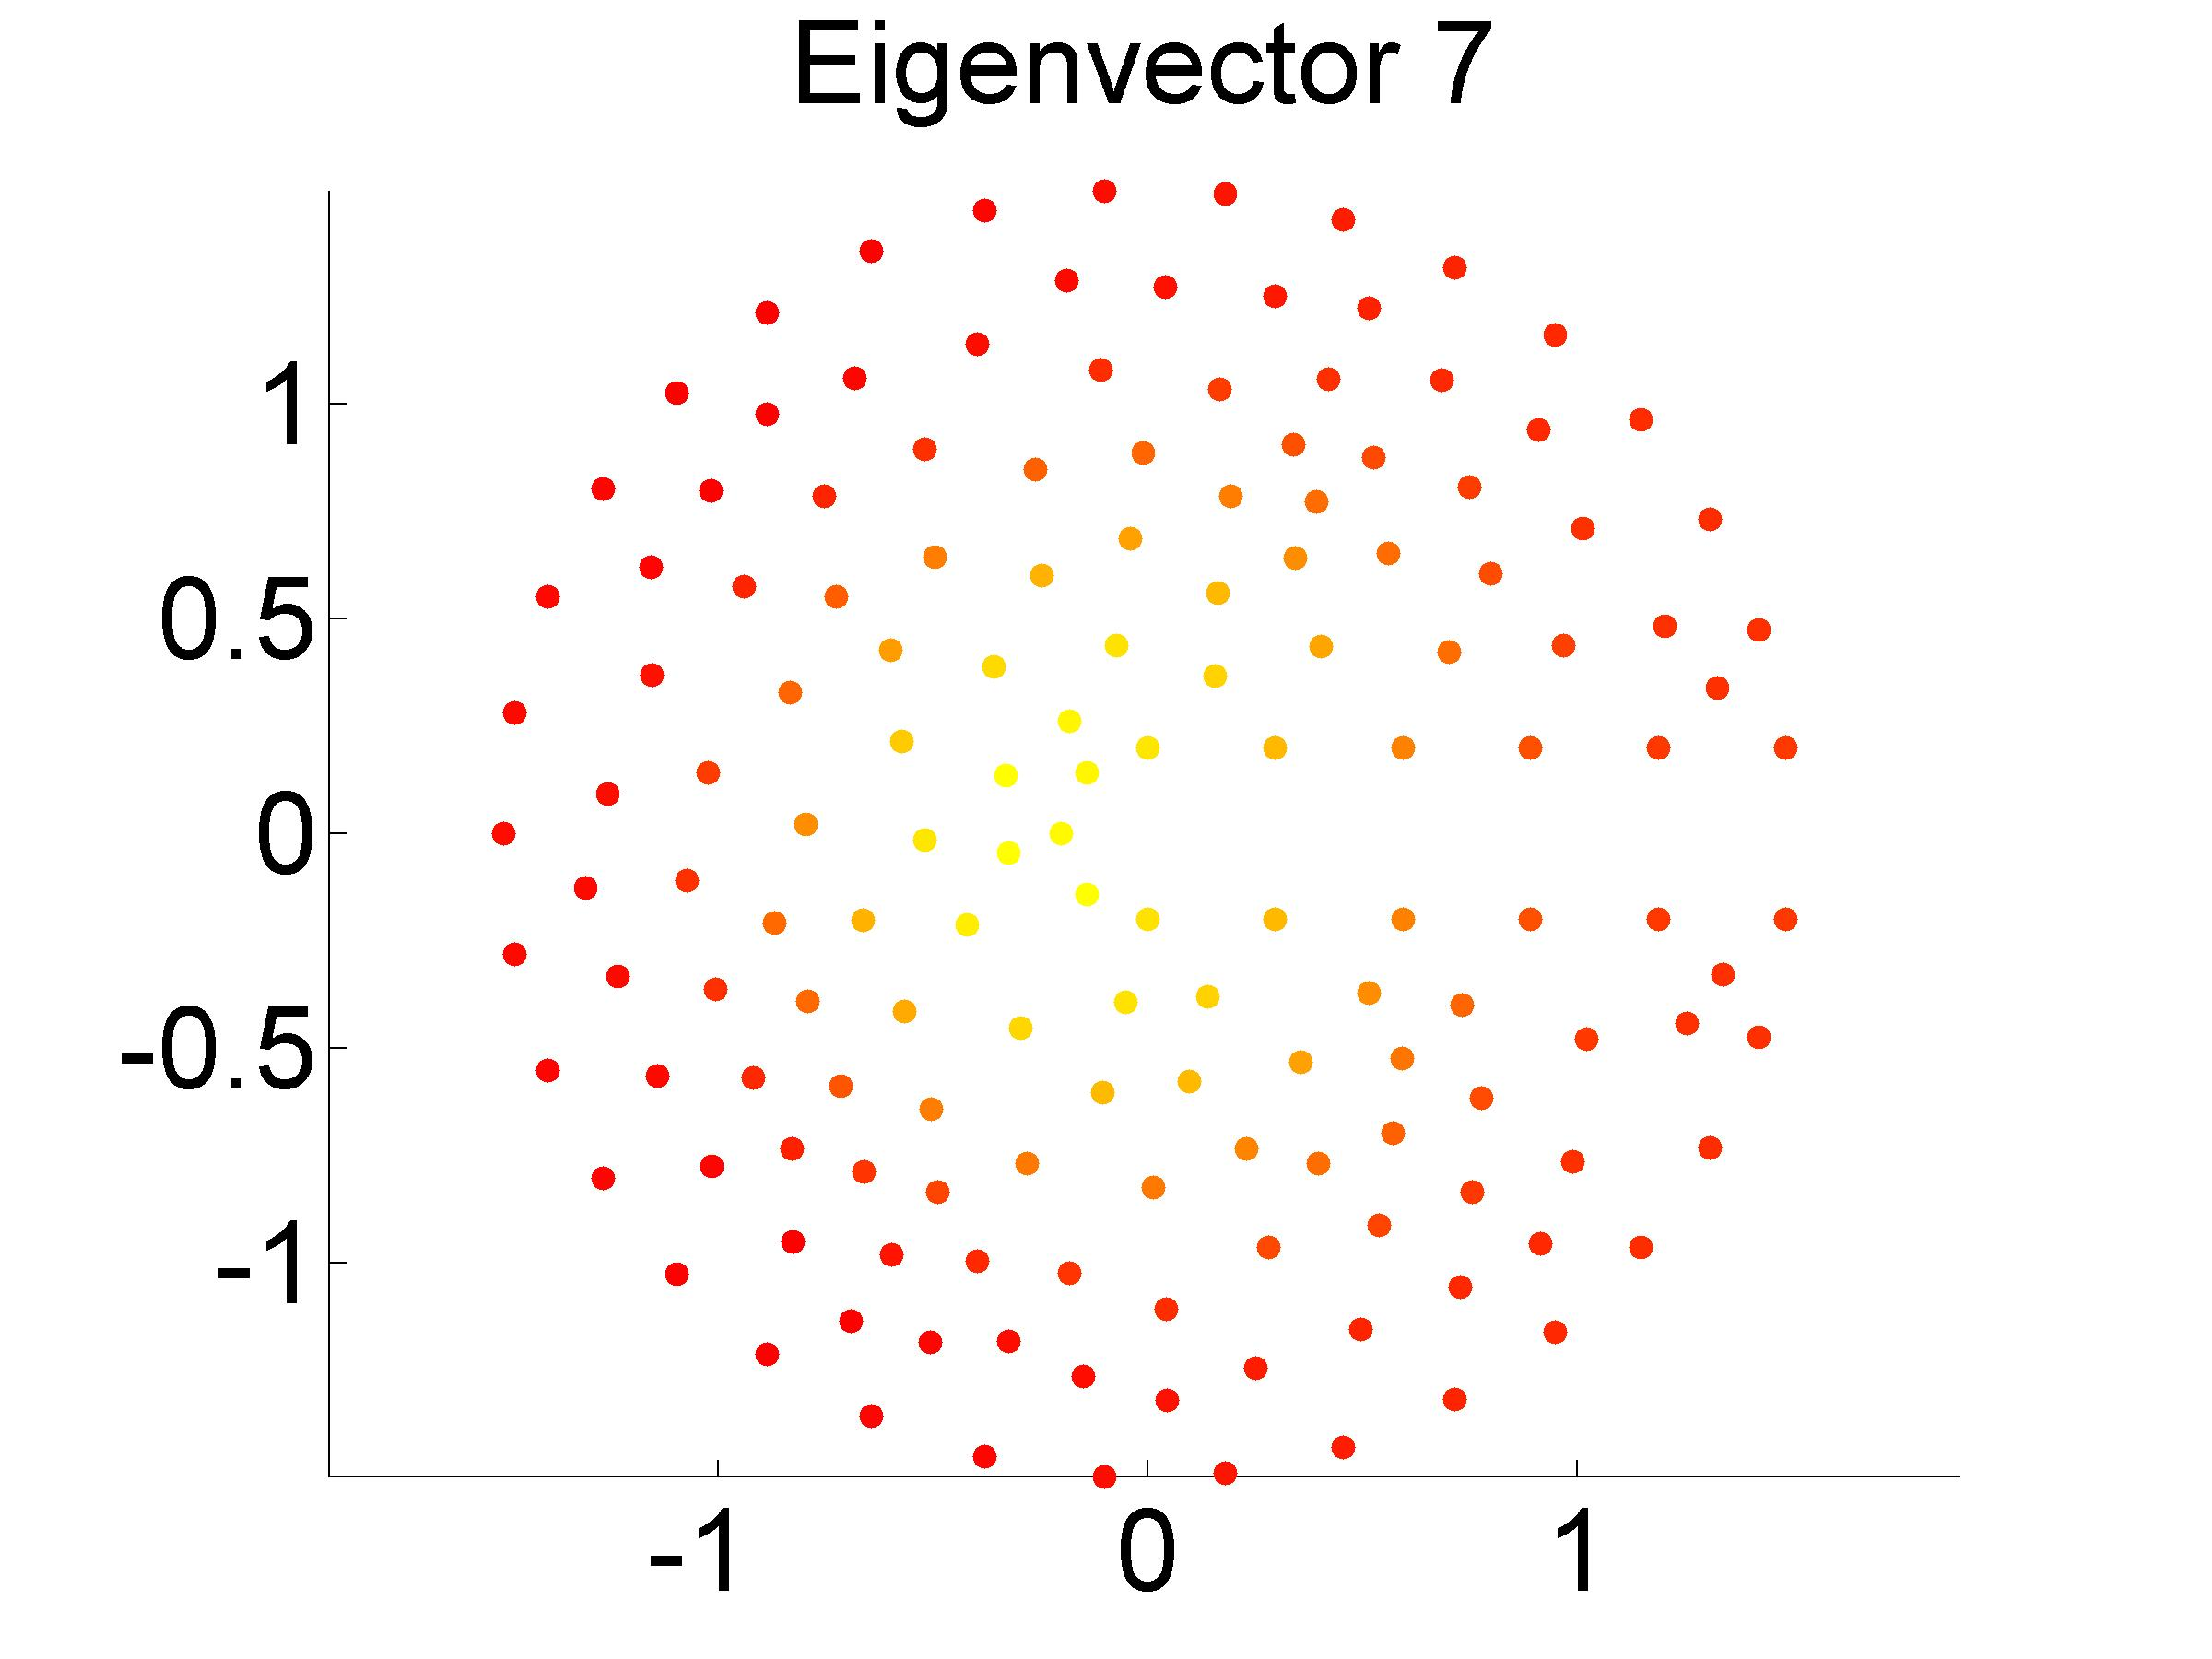
\includegraphics[width=0.18\textwidth]{circle_evec6.jpg}\\

    \vspace{0.05in}

    {\small Diffusion maps approximates the eigenfunctions for a manifold \\ using data sampled from the manifold \par}

\end{frame}

\begin{frame}{DMAPS Implementation }

	\newfootnote{Coifman {\em et al}, PNAS, 2005}
	
    \begin{itemize}
    {\small
        \item Assume we have data $y_1, y_2, \dots, y_n \in \mathbb{R}^d$ that are sampled 		\\from an underlying manifold $\mathcal{M}$
        \item We have a {\bf distance metric} $d(y_i, y_j)$ for our data
        \item We construct the matrix $W \in \mathbb{R}^{n \times n}$, with
        $$W_{ij} = \exp \left( -\frac{d^2 (x_i, x_j)}{\sigma_{kernel}^2} \right) $$
        where $\sigma_{kernel}$ is a characteristic distance 
        %\leavevmode\makebox(0,0){\put(60, 70){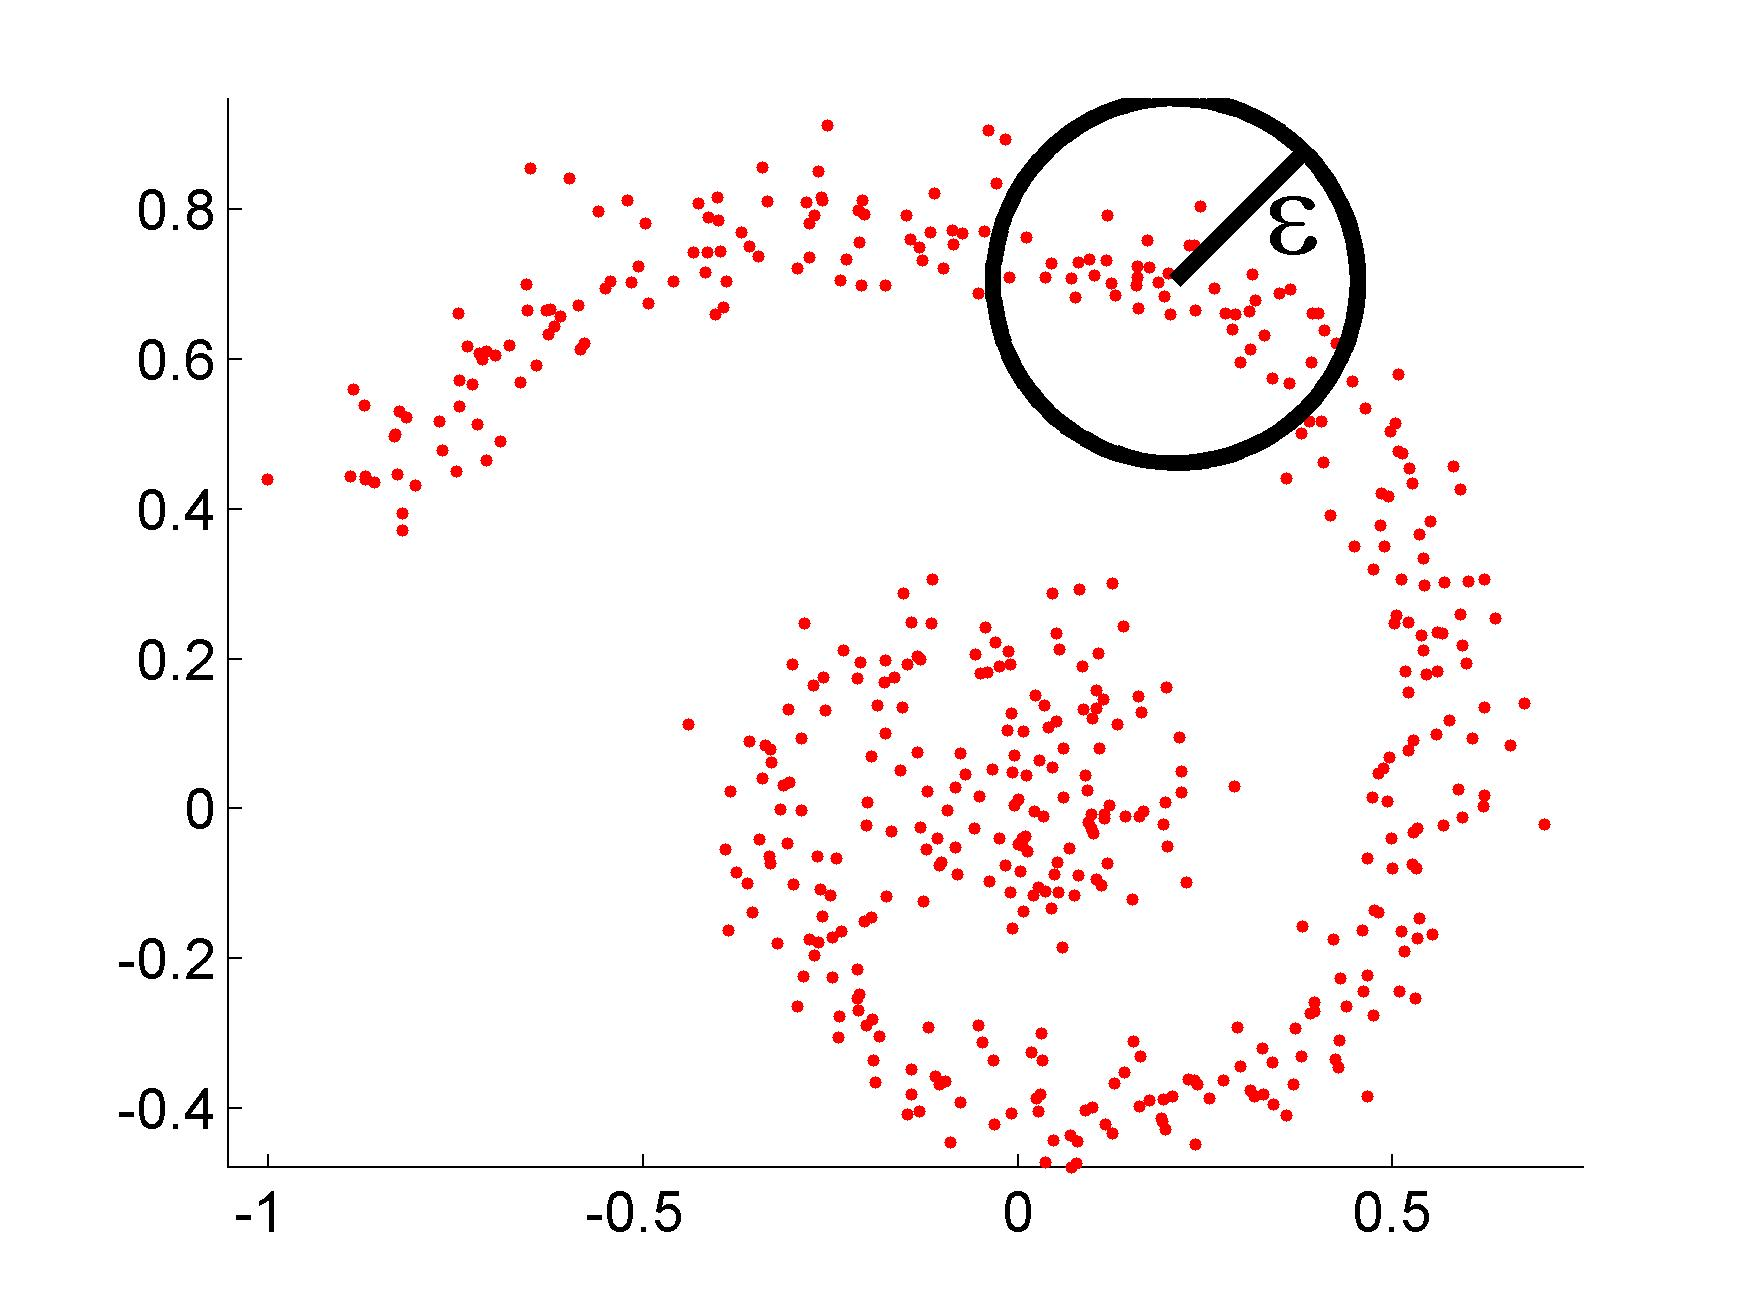
\includegraphics[width=0.25\textwidth]{spiral_with_ball.jpg}}}

        \item We define the diagonal matrix $D$ with $D_{ii} = \sum_{j=1}^{n} W_{ij}$, \\
        and the matrix $A =  D^{-1} W$, where $A$ is a Markov transition matrix

        \item $I-A$ then approximates the Laplacian on the manifold $\mathcal{M}$

        \item We compute the {\em real} {\bf eigenvectors} $\phi_0, \phi_1, \dots, \phi_{n-1}$ and \\{\bf eigenvalues} $\lambda_0, \lambda_1, \dots, \lambda_{n-1}$ of $A$

        %\item We {\bf order} the eigenvector/eigenvalue pairs such that $|\lambda_1| \ge |\lambda_2| \ge \dots \ge |\lambda_n|$

        \item The eigenvectors then approximate the eigenfunctions \\of the Laplacian {\em on the manifold} $\mathcal{M}$
        \par}
    \end{itemize}
	

\end{frame}

\begin{frame}{Data-Driven Reduction for Multiscale Data}

{\bf Issue:} Direction of largest variance is not necessarily the {\em slow} direction

\begin{center}
\begin{tikzpicture}
\node(a){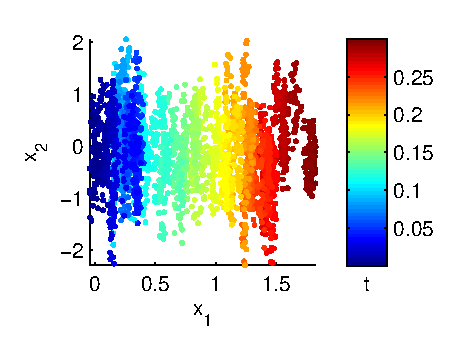
\includegraphics[width=6cm]{data_init}};
\draw[->, red] (-2,-2.25) -- (1,-2.25) node [draw=none,midway,below=0cm, red] {Slow direction};
\draw[->, red] (-3.5,-2) -- (-3.5,2) node [draw=none,midway,left=0cm, rotate=90,red, anchor=center, align=center] {Fast direction\\ Large variance};
\end{tikzpicture}
\end{center}
%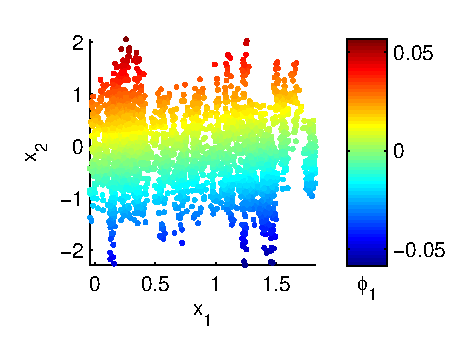
\includegraphics[width=0.5\textwidth]{data_linear_DMAPS}

We will construct a {\em more informative metric} which captures the relative time scales in the data

\end{frame}

\begin{frame}{Mahalanobis Distance: A Good Metric}

\begin{block}{Mahalanobis distance, $\| \cdot \|_M$}
$$\| \vec{x}(t_2) - \vec{x}(t_1) \|^2_M = \| \vec{z}(t_2) - \vec{z}(t_1) \|^2_2$$
where $\vec{z}$ obey the following SDEs
$$dz_i(t) = b_i(\vec{z}(t)) dt + dW_i(t)$$
\end{block}

\end{frame}

\begin{frame}{Mahalanobis Distance: A Good Metric}



For the multiscale SDE we are considering,

\begin{tikzpicture}

\node[fill=orange!20](a) {$\begin{aligned}
dx_i(t) &= a_i(\vec{x}(t)) dt + dW_i(t), & \: 1 \le i \le m \\
dx_i(t) &= \frac{a_i(\vec{x}(t))}{\epsilon} dt + \frac{1}{\sqrt{\epsilon}} dW_i(t) , & \: m+1 \le i \le n
\end{aligned}$};

\node[below=3cm of a,fill=orange!20](b) {$dz_i(t) = b_i(\vec{z}(t)) dt + dW_i(t)$};

\node[align=center,below right=0.5cm and -4.5cm of a, fill=yellow!20](c) {Rescale $x_{m+1}, \dots, x_n$  by $\sqrt{\epsilon}$ \\{\small $\begin{aligned}
z_i &= x_i, & \: 1 \le i \le m \\
z_i &= \sqrt{\epsilon}x_i , & \: m+1 \le i \le n
\end{aligned}$}};

\draw[->](a) -- (b);

\end{tikzpicture}


%\begin{equation*}
%\begin{aligned}
%dx_i(t) &= a_i(\vec{x}(t)) dt + dW_i(t), & \: 1 \le i \le m \\
%dx_i(t) &= \frac{a_i(\vec{x}(t))}{\epsilon} dt + \frac{1}{\sqrt{\epsilon}} dW_i(t) , & \: m+1 \le i \le n
%\end{aligned}
%\end{equation*}
%this amounts to . 


\end{frame}

\begin{frame}{Mahalanobis Distance Collapses Fast Directions}

\begin{tikzpicture}
\node[fill=orange!20](a) {{\small $\begin{aligned} 
\| \vec{x}(t_2) - \vec{x}(t_1) \|^2_M  &= \| \vec{z}(t_2) - \vec{z}(t_1) \|^2_2 \\
&= \sum_{i=1}^n \left( z_i(t_2) - z_i(t_1) \right)^2 \\
&= \sum_{i=1}^m  \left( x_i(t_2) - x_i(t_1) \right)^2 + \underbrace{\sum_{i=m+1}^n \epsilon \left( x_i(t_2) - x_i(t_1) \right)^2}
\end{aligned}$}};

\node[align=center,below left=0cm and -5cm of a, fill=yellow!20](c) {{\scriptsize $\begin{aligned}
z_i &= x_i, & \: 1 \le i \le m \\
z_i &= \sqrt{\epsilon}x_i , & \: m+1 \le i \le n
\end{aligned}$}};

\node[align=center,below right=1cm and -5cm of a, fill=yellow!20, text width=4cm](d) {Fast variables are scaled by $\epsilon$!};

\draw[->](c.north) -- (-2.5,-1.1);
\draw[->](d.north) -- (3.75,-1.75);

\end{tikzpicture}

\end{frame}


\begin{frame}{Nonlinear Data}

\begin{block}

We could have data
$$\vec{y} = \mathbf{f}(\vec{x})$$
where $\mathbf{f}$ is some nonlinear measurement function. 
\end{block}

\newfootnote{Coifman and Singer, ACHA, 2009}


Mahalanobis distance is invariant (to fourth order) to nonlinear transformations!

$$\| \vec{y}(t_2) - \vec{y}(t_1) \|^2_M = \| \vec{z}(t_2) - \vec{z}(t_1) \|^2_2 + \mathcal{O}(\|  \vec{y}(t_2) - \vec{y}(t_1) \|^4_2)$$

\end{frame}

\begin{frame}{Recap: General Setup}


\begin{itemize}

\item We have data $\vec{y}(t_1), \vec{y}(t_2), \dots, \vec{y}(t_N)$


\item $\vec{y} = \mathbf{f}(\vec{x})$, where $\mathbf{f}$ is some nonlinear function


\item $\vec{x}$ comes from a multiscale SDE


\item $\vec{z}$ is the {\em rescaled} verson of $\vec{x}$ which collapses the fast directions



\end{itemize}


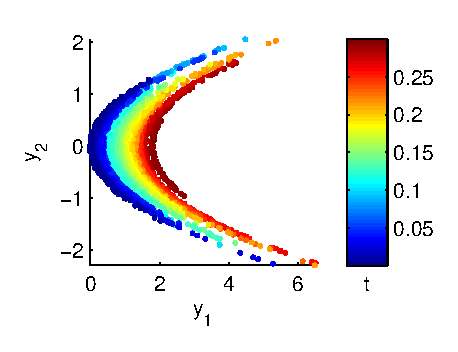
\includegraphics[width=0.3\textwidth]{data_init_nonlinear}
\hfill
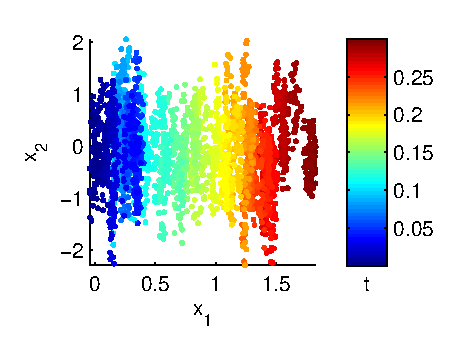
\includegraphics[width=0.3\textwidth]{data_init}
\hfill
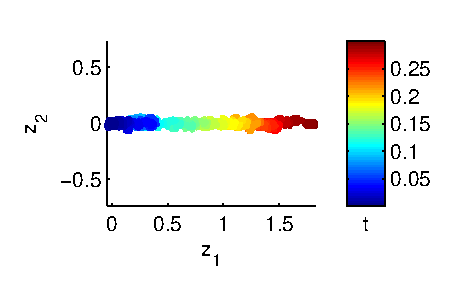
\includegraphics[width=0.3\textwidth]{data_rescaled}

We want to recover a parameterization of the data $\vec{y}(t_1), \vec{y}(t_2), \dots, \vec{y}(t_N)$ which respects the {\em slow variables}

\end{frame}

\section{Error Analysis}

%\begin{frame}{General Error Terms}
%
%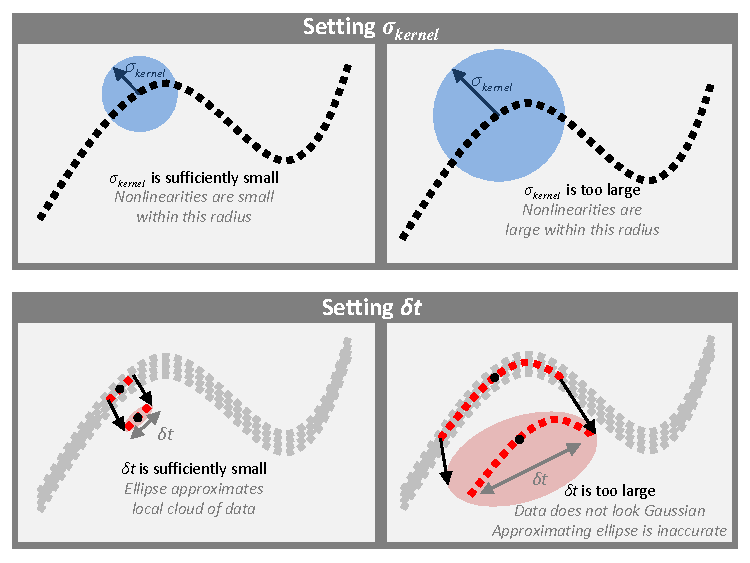
\includegraphics[width=0.7\textwidth]{schematic}
%
%\begin{enumerate}
%
%\item Error from Taylor expansion
%
%\item Error from covariance estimation
%
%\end{enumerate}
%
%\end{frame}

\begin{frame}{Errors in Mahalanobis Distance}

Goal: write $\| \vec{z}(t_2) - \vec{z}(t_1) \|$ in terms of $\vec{y}(t_1), \vec{y}(t_2)$

Let $\mathbf{g} = \mathbf{f}^{-1}$. By Taylor expansion of $\mathbf{g}(y)$,
%
\begin{tikzpicture}
\node[fill=orange!20](a) { {\scriptsize $
\begin{aligned}
\| \vec{z}(t_2) - \vec{z}(t_1) \|^2_2 =&
\overbrace{\frac{1}{2} \left(\vec{y}(t_2)-\vec{y}(t_1)\right)^T \left(C^\dagger (\vec{y}(t_1)) + C^\dagger (\vec{y}(t_2)) \right) (\vec{y}(t_2)-\vec{y}(t_1))} \\
&+ \underbrace{ E_M \left(\vec{y}(t_1), \vec{y}(t_2) \right)} + \underbrace{ \mathcal{O} \left(\| \vec{y}(t_2) - \vec{y}(t_1) \|^6_2 \right)}
\end{aligned}
$}};

\node[above=0.5cm of a, fill=yellow!20, align=center, text width=6cm](text1){{\small Mahalanobis distance\\$C$ is the covariance of $\vec{y}$ \\$\dagger$ denotes the pseudoinverse \par}};

\node[below left=0.5cm and -6cm of a, fill=yellow!20, align=center, text width=6cm](text2){{\small $\mathcal{O} \left(\| \vec{y}(t_2) - \vec{y}(t_1) \|^4_2 \right)$ error term\\ Involves second- and higher-order derivatives of $\mathbf{g}$ \par}};

\node[below right=0.5cm and -4cm of a, fill=yellow!20, align=center, text width=4cm](text3){{\small Higher-order error term}};


\draw[->] (text1.south) -- (1.1,0.8);
\draw[->] (text2.north) -- (-1.2,-0.8);
\draw[->] (text3.north) -- (1.6,-0.8);

\end{tikzpicture}

%\begin{equation}
%\begin{aligned} 
%E_M\left( \vec{y}(t_1), \vec{y}(t_2) \right)
% =
%\frac{1}{2} \sum_{i=1}^n \sum_{jkl=1}^{d} &
%\left( g_{i, (j)} (\vec{y}(t_1)) g_{i, (k,l)} (\vec{y}(t_1)) -  g_{i, (j)} (\vec{y}(t_2)) g_{i, (k,l)} (\vec{y}(t_2)) \right) \\
%& (\vec{y}_j(t_2) - \vec{y}_j(t_1))   (\vec{y}_k(t_2) - \vec{y}_k(t_1))(\vec{y}_l(t_2) - \vec{y}_l(t_1)) \\
%+ \frac{1}{8} \sum_{i=1}^n \sum_{jklm=1}^d  &
%\left( g_{i, (j,k)} (\vec{y}(t_1)) g_{i, (l,m)} (\vec{y}(t_1)) +  g_{i, (j,k)} (\vec{y}(t_2)) g_{i, (l,m)} (\vec{y}(t_2)) \right) \\
%&(\vec{y}_j(t_2) - \vec{y}_j(t_1))  (\vec{y}_k(t_2) - \vec{y}_k(t_1))(\vec{y}_l(t_2) - \vec{y}_l(t_1)) (\vec{y}_m(t_2) - \vec{y}_m(t_1)) \\
%+ \frac{1}{6} \sum_{i=1}^n \sum_{jklm=1}^d &
%\left( g_{i, (j)} (\vec{y}(t_1)) g_{i, (k,l,m)} (\vec{y}(t_1)) +  g_{i, (j)} (\vec{y}(t_2)) g_{i, (k,l,m)} (\vec{y}(t_2)) \right) \\
%& (\vec{y}_j(t_2) - \vec{y}_j(t_1))  (\vec{y}_k(t_2) - \vec{y}_k(t_1))(\vec{y}_l(t_2) - \vec{y}_l(t_1))(\vec{y}_m(t_2) - \vec{y}_m(t_1))
%\end{aligned}
%\end{equation}
%%
%where
%%
%\begin{equation}
%\begin{aligned}
%g_{i,(j)} &= \sqrt{e_i} \frac{\partial g_i}{\partial y_j}
%\\
%g_{i,(j,k)} &= \sqrt{e_i}  \frac{\partial^2 g_i}{\partial y_j \partial y_k}
%\\
%g_{i,(j,k,l)} &= \sqrt{e_i}  \frac{\partial^3 g_i}{\partial y_j \partial y_k \partial y_l}
%\end{aligned}
%\end{equation}

\end{frame}

\begin{frame}{Setting the Kernel Scale}

\begin{tikzpicture}
\node[fill=orange!20](a) { {\scriptsize $
\begin{aligned}
\| \vec{z}(t_2) - \vec{z}(t_1) \|^2_2 =&
{\frac{1}{2} \left(\vec{y}(t_2)-\vec{y}(t_1)\right)^T \left(C^\dagger (\vec{y}(t_1)) + C^\dagger (\vec{y}(t_2)) \right) (\vec{y}(t_2)-\vec{y}(t_1))} \\
&+ { E_M \left(\vec{y}(t_1), \vec{y}(t_2) \right)} + { \mathcal{O} \left(\| \vec{y}(t_2) - \vec{y}(t_1) \|^6_2 \right)}
\end{aligned}
$}};

\node[below=0cm of a](b){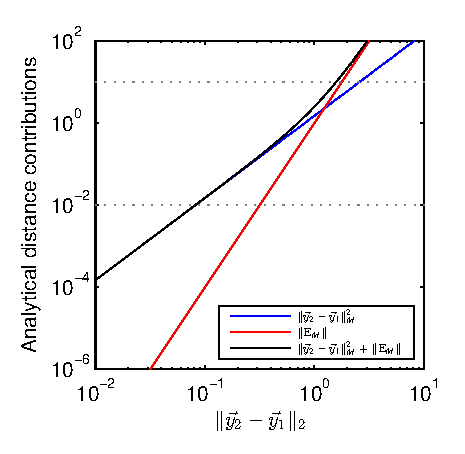
\includegraphics[width=0.5\textwidth]{dist_dy_analytical_nonlinear}};

\node[right=0.5cm of b, text width=4cm](text1){{\scriptsize Mahalanobis distance dominates\par}};
\node[above right=-1cm and 0.5cm of b, text width=4cm](text2){{\scriptsize Errors dominate \par}};

\draw[->] (text1.west) -- (2.5,-3.25);
\draw[->] (text2.west) -- (2.5,-1.65);

\end{tikzpicture}

\vspace{-0.25cm}
Want to choose kernel scale $\sigma_{kernel}$ \\such that Mahalanobis distance dominates
%
%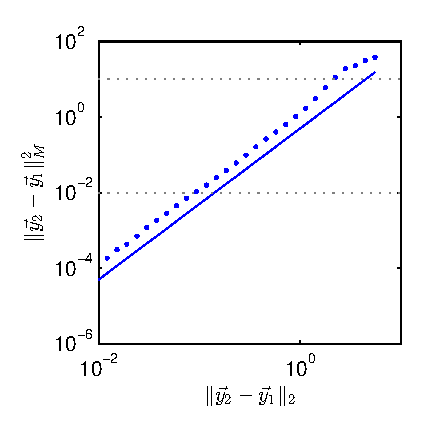
\includegraphics[width=0.5\textwidth]{dist_dy_nonlinear}

\end{frame}

\begin{frame}{Setting the Kernel Scale Empirically}

\begin{tikzpicture}
\node[fill=orange!20](a) { {\scriptsize $
\begin{aligned}
\| \vec{z}(t_2) - \vec{z}(t_1) \|^2_2 =&
{\frac{1}{2} \left(\vec{y}(t_2)-\vec{y}(t_1)\right)^T \left(C^\dagger (\vec{y}(t_1)) + C^\dagger (\vec{y}(t_2)) \right) (\vec{y}(t_2)-\vec{y}(t_1))} \\
&+ { E_M \left(\vec{y}(t_1), \vec{y}(t_2) \right)} + { \mathcal{O} \left(\| \vec{y}(t_2) - \vec{y}(t_1) \|^6_2 \right)}
\end{aligned}
$}};

\node[below=0cm of a](b){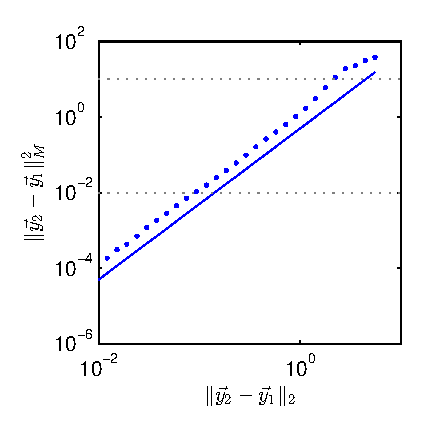
\includegraphics[width=0.5\textwidth]{dist_dy_nonlinear}};

\node[right=0.5cm of b, text width=4cm](text1){{\scriptsize Mahalanobis distance dominates\par}};
\node[above right=-1cm and 0.5cm of b, text width=4cm](text2){{\scriptsize Errors dominate \par}};

\draw[->] (text1.west) -- (2.5,-3.25);
\draw[->] (text2.west) -- (2.5,-1.65);

\end{tikzpicture}

Want $\| \vec{y}_2 - \vec{y}_1 \|^2_M \propto \| \vec{y}_2 - \vec{y}_1 \|^2_2$

\end{frame}


\begin{frame}{Errors from covariance estimation}

By It\={o}-Taylor expansion of $\mathbf{f}$ and $\vec{x}(t)$,

\makebox[\textwidth][c]{
\begin{tikzpicture}
\node[fill=orange!20](a) { {\scriptsize $
\begin{aligned}
\hat{C}_{ij} (\vec{x}_t, \delta t)
=&
\overbrace{\frac{1}{\delta t} \left( \mathbb{E} \left[ y_i (t+\delta t) y_j (t+ \delta t) \mid \vec{y}(t) \right]
- \mathbb{E} \left[ y_i (t+\delta t) \mid \vec{y}(t) \right] \mathbb{E} \left[ y_j (t+\delta t) \mid \vec{y}(t) \right] \right)}
\\
=& \underbrace{\sum_{k=1}^m \left. \frac{\partial f_{i}}{\partial x_k} \right|_{\vec{x}(t)} \left. \frac{\partial f_{j}}{\partial x_k} \right|_{\vec{x}(t)}
+ \frac{1}{\sqrt{\epsilon}} \sum_{k=m+1}^n  \left. \frac{\partial f_{i}}{\partial x_k} \right|_{\vec{x}(t)} \left. \frac{\partial f_{j}}{\partial x_k} \right|_{\vec{x}(t)}}
+ \underbrace{E_{C, ij} (\vec{x}(t), \delta t)} + \underbrace{\mathcal{O}(\delta t^{3/2})}
\end{aligned}
$}};

\node[above=0.5cm of a, fill=yellow!20, align=center, text width=6cm](text1){{\small Empirically estimate local covariance \par}};

\node[below left=0.5cm and -3cm of a, fill=yellow!20, align=center, text width=3cm](text2){{\small True covariance \par}};

\node[below=0.5cm of a, fill=yellow!20, align=center, text width=4cm](text3){{\small $\mathcal{O} (\delta t)$ error term \\ Depends on drift, and second- and higher-order derivatives of $\mathbf{f}$  \par}};

\node[below right=0.5cm and -3cm of a, fill=yellow!20, align=center, text width=3	cm](text4){{\small $\mathcal{O} (\delta t^{3/2})$ error term}};

\draw[->] (text1.south) -- (0.6,1.1);
\draw[->] (text2.north) -- (-0.9,-1.1);
\draw[->] (text3.north) -- (3.5,-0.8);
\draw[->] (text4.north) -- (5.25,-0.8);

\end{tikzpicture}
}

%\begin{equation}\label{eq:estimated_cov}
%\begin{aligned}
%\hat{C}_{ij} (\vec{x}_t, \delta t)
%=&
%\frac{1}{\delta t} \left( \mathbb{E} \left[ y_i (t+\delta t) y_j (t+ \delta t) \mid \vec{y}(t) \right]
%- \mathbb{E} \left[ y_i (t+\delta t) \mid \vec{y}(t) \right] \mathbb{E} \left[ y_j (t+\delta t) \mid \vec{y}(t) \right] \right)
%\\
%=& \sum_{k=1}^n \frac{1}{e_k} \left. \frac{\partial f_{i}}{\partial x_k} \right|_{\vec{x}(t)} \left. \frac{\partial f_{j}}{\partial x_k} \right|_{\vec{x}(t)}
%+ E_{C, ij} (\vec{x}(t), \delta t) + \mathcal{O}(\delta t^{3/2})
%%=& \sum_{k=1}^n \frac{1}{e_k} \left. \frac{\partial f_{i}}{\partial x_k} \right|_{\vec{x}(t)} \left. \frac{\partial f_{j}}{\partial x_k} \right|_{\vec{x}(t)} \\
%%&+ \frac{1}{\delta t} \sum_{k=1}^n f_{i,(k)}(\vec{x}(t)) \left( \mathbb{E} \left[ \int_t^{t+\delta t} \int_{s_1}^{t+\delta t} f_{j,(k,0)}(\vec{x}(s_2)) ds_2 ds_1 \right]
%%+ \mathbb{E} \left[  \int_t^{t+\delta t} \int_t^{s_2} f_{j,(0,k)}(\vec{x}(s_1)) ds_1 ds_2\right] \right) \\
%%&+  \frac{1}{\delta t} \sum_{k=1}^n f_{j,(k)}(\vec{x}(t)) \left( \mathbb{E} \left[ \int_t^{t+\delta t} \int_{s_1}^{t + \delta t} f_{i,(k,0)}(\vec{x}(s_2)) ds_2 ds_1 \right]
%%+ \mathbb{E} \left[ \int_t^{t+\delta t} \int_t^{s_2} f_{i,(0,k)}(\vec{x}(s_1)) ds_1 ds_2 \right] \right) \\
%%&+  \frac{1}{\delta t} \sum_{k,l=1}^n \mathbb{E} \left[ \int_t^{t+\delta t}\left( \int_t^{s_2} f_{i,(k,l)}(\vec{x}(s_1)) dW_{s_1, k}  \right) \left(  \int_t^{s_2} f_{j,(k,l)}(\vec{x}(s_1)) dW_{s_1, k} \right) ds_2 \right] \\
%%&+ \mathcal{O} (\delta t^{3/2}),
%\end{aligned}
%\end{equation}
%%
%where $E_C = \mathcal{O} (\delta t)$ is an error term, with
%%
%\begin{equation} \label{eq:cov_error}
%\begin{aligned}
%E_{C, ij} (\vec{x}(t), \delta t) =&
% \frac{1}{\delta t} \sum_{k=1}^n f_{i,(k)}(\vec{x}(t)) \mathbb{E} \left[ \int_t^{t+\delta t} \left( \int_{s_2}^{t+\delta t} f_{j,(k,0)}(\vec{x}(s_1)) ds_1
%+ \int_t^{s_2} f_{j,(0,k)}(\vec{x}(s_1)) ds_1 \right) ds_2 \right] \\
%&+  \frac{1}{\delta t} \sum_{k=1}^n f_{j,(k)}(\vec{x}(t))  \mathbb{E} \left[ \int_t^{t+\delta t} \left( \int_{s_2}^{t + \delta t} f_{i,(k,0)}(\vec{x}(s_1)) ds_1
%+  \int_t^{s_2} f_{i,(0,k)}(\vec{x}(s_1)) ds_1 \right) ds_2 \right] \\
%&+  \frac{1}{\delta t} \sum_{k,l=1}^n \mathbb{E} \left[ \int_t^{t+\delta t}\left( \int_t^{s_2} f_{i,(k,l)}(\vec{x}(s_1)) dW_{s_1, k}  \right) \left(  \int_t^{s_2} f_{j,(k,l)}(\vec{x}(s_1)) dW_{s_1, k} \right) ds_2 \right]
%\end{aligned}
%\end{equation}

\end{frame}

\begin{frame}{Setting the Covariance Timescale}

\makebox[\textwidth][c]{
\begin{tikzpicture}
\node[fill=orange!20](a) { {\scriptsize $
\hat{C}_{ij} (\vec{x}_t, \delta t)
= {\sum_{k=1}^m \left. \frac{\partial f_{i}}{\partial x_k} \right|_{\vec{x}(t)} \left. \frac{\partial f_{j}}{\partial x_k} \right|_{\vec{x}(t)}
+ \frac{1}{\sqrt{\epsilon}} \sum_{k=m+1}^n  \left. \frac{\partial f_{i}}{\partial x_k} \right|_{\vec{x}(t)} \left. \frac{\partial f_{j}}{\partial x_k} \right|_{\vec{x}(t)}}
+ {E_{C, ij} (\vec{x}(t), \delta t)} + {\mathcal{O}(\delta t^{3/2})}
$}};

\node[below=1cm of a](b){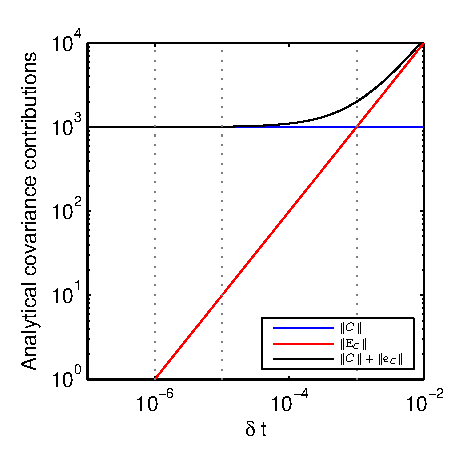
\includegraphics[width=0.5\textwidth]{C_dt_analytical_linear}};

\node[above left=0.25cm and -2cm of b](text1){True covariance dominates};
\node[right=3cm of text1](text2){Errors dominate};

\draw[->] (text1.south) --  (-1,-1.8);
\draw[->] (text1.south) --  (-0.1,-1.8);
\draw[->] (text2.south) --  (1.5,-1.8);

\end{tikzpicture}
}

\vspace{-0.25cm}
Want to choose $\delta t$ such that true covariance dominates

\end{frame}

\begin{frame}{Setting the Covariance Timescale Empirically}

\makebox[\textwidth][c]{
\begin{tikzpicture}
\node[fill=orange!20](a) { {\scriptsize $
\hat{C}_{ij} (\vec{x}_t, \delta t)
= {\sum_{k=1}^m \left. \frac{\partial f_{i}}{\partial x_k} \right|_{\vec{x}(t)} \left. \frac{\partial f_{j}}{\partial x_k} \right|_{\vec{x}(t)}
+ \frac{1}{\sqrt{\epsilon}} \sum_{k=m+1}^n  \left. \frac{\partial f_{i}}{\partial x_k} \right|_{\vec{x}(t)} \left. \frac{\partial f_{j}}{\partial x_k} \right|_{\vec{x}(t)}}
+ {E_{C, ij} (\vec{x}(t), \delta t)} + {\mathcal{O}(\delta t^{3/2})}
$}};

\node[below=1cm of a](b){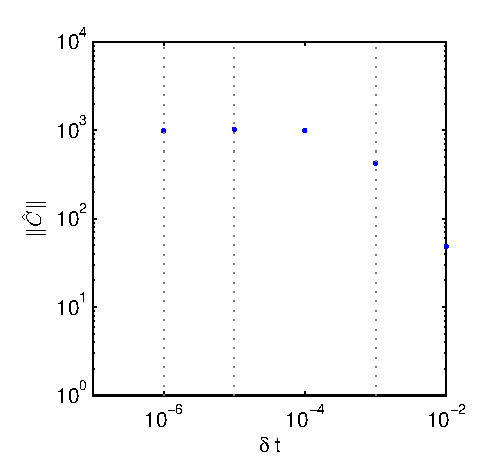
\includegraphics[width=0.5\textwidth]{C_dt_linear}};

\node[above left=0.25cm and -2cm of b](text1){True covariance dominates};
\node[right=3cm of text1](text2){Errors dominate};

\draw[->] (text1.south) --  (-1,-1.8);
\draw[->] (text1.south) --  (-0.1,-1.8);
\draw[->] (text2.south) --  (1.5,-1.8);

\end{tikzpicture}
}

\vspace{-0.25cm}
Find where $\hat{C}$ is constant with respect to $\delta t$

\end{frame}

\section{Examples}

\begin{frame}{Linear Two-Dimensional Data}

\begin{block}{}	
\begin{equation*} 
\begin{aligned}
dx_1(t) &=& adt &+& dW_1(t)\\
dx_2(t) &=& -\frac{x_2(t)}{\epsilon} dt &+& \frac{1}{\sqrt{\epsilon}} dW_2(t)
\end{aligned}
\end{equation*} 
\end{block}

\centering
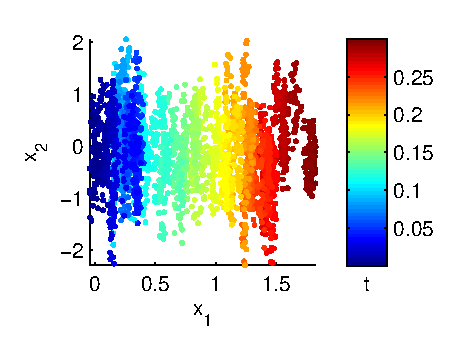
\includegraphics[width=0.45\textwidth]{data_init}

$x_1$ is the slow variable, $x_2$ is the fast variable \newfootnote{$a=3$, $\epsilon = 10^{-3}$}

\end{frame}

\begin{frame}{Reduction of Linear Data}

\begin{tikzpicture}
\node(a){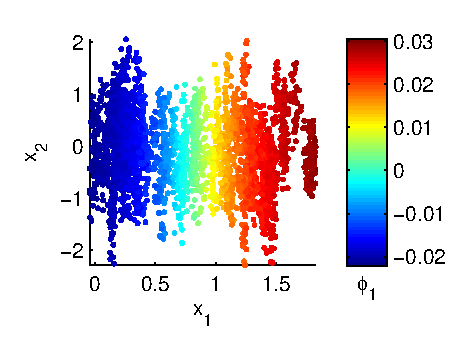
\includegraphics[width=0.5\textwidth]{data_linear_NIV}};
\node[right=0cm of a](b){ 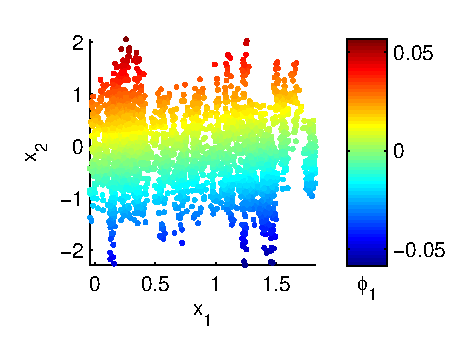
\includegraphics[width=0.5\textwidth]{data_linear_DMAPS}};

\node[above=0cm of a, text width=0.45\textwidth, align=center](texta1){Using Mahalanobis distance};
\node[below=0cm of a, text width=0.4\textwidth, align=center](texta2){{\scriptsize Parameterization is consistent with slow variable $x_1$ \par}};

\node[above=0cm of b, text width=0.4\textwidth, align=center](textb1){Using Euclidean distance};
\node[below=0cm of b, text width=0.4\textwidth, align=center](textb2){{\scriptsize Parameterization is inconsistent with slow variable $x_1$ \par}};

\end{tikzpicture}

\end{frame}

\begin{frame}{Curved ``Half-Moon'' Data}

\begin{block}{}
\begin{equation*}
\begin{aligned}
dx_1(t) =& adt + dW_1(t)\\
dx_2(t) =& -\frac{x_2(t)}{\epsilon} dt + \frac{1}{\sqrt{\epsilon}} dW_2(t)\\
\begin{bmatrix}
y_1(t) \\ y_2(t)
\end{bmatrix} =&
\mathbf{f}(\vec{x}(t)) =
\begin{bmatrix}
x_1(t) + x_2^2(t) \\
x_2(t)
\end{bmatrix}
\end{aligned}
\end{equation*}
\end{block}

\centering
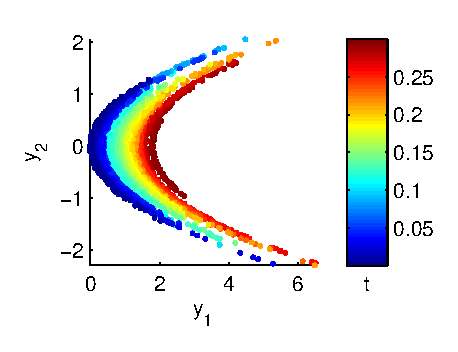
\includegraphics[width=0.5\textwidth]{data_init_nonlinear}

\end{frame}

\begin{frame}{Reduction of Nonlinear Data}

\begin{tikzpicture}

\node(a){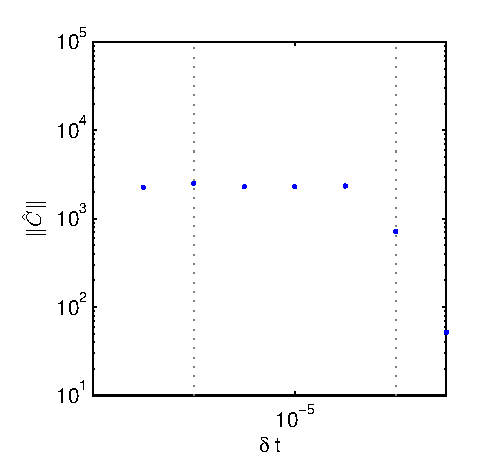
\includegraphics[width=0.3\textwidth]{C_dt_nonlinear}};
\node[below=0cm of a](b){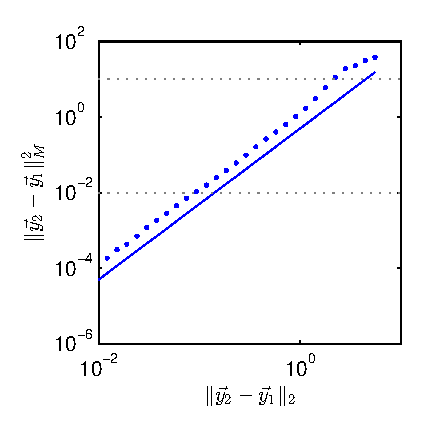
\includegraphics[width=0.3\textwidth]{dist_dy_nonlinear}};

\node[below right=-3cm and 1cm of a, align=center, text width=0.5\textwidth](c){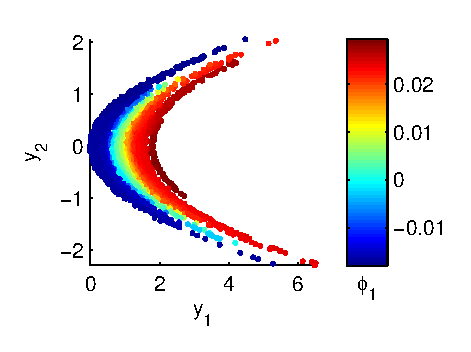
\includegraphics[width=\textwidth]{data_nonlinear_NIV_dt1_kernel1} \\ Using an appropriate value of $\delta t$ and $\sigma_{kernel}$};

\draw[->, red] (-0.35, 1.7) -- (-0.35,1.45);
\draw[->, red] (1.85, -3.35) -- (1.6,-3.35);

\end{tikzpicture}

\end{frame}

\begin{frame}{Reduction of Nonlinear Data}

\begin{tikzpicture}

\node(a){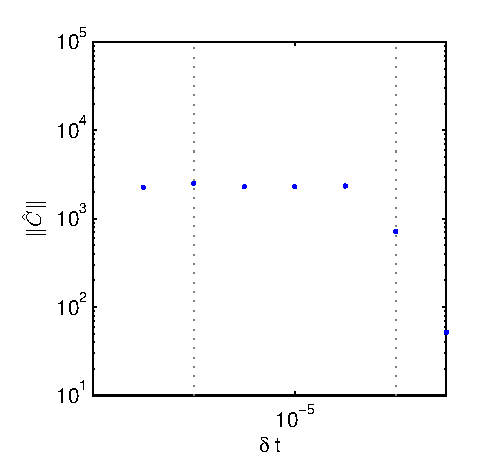
\includegraphics[width=0.3\textwidth]{C_dt_nonlinear}};
\node[below=0cm of a](b){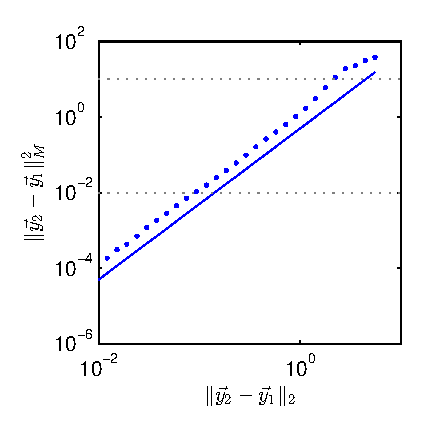
\includegraphics[width=0.3\textwidth]{dist_dy_nonlinear}};

\node[below right=-3cm and 1cm of a, align=center, text width=0.5\textwidth](c){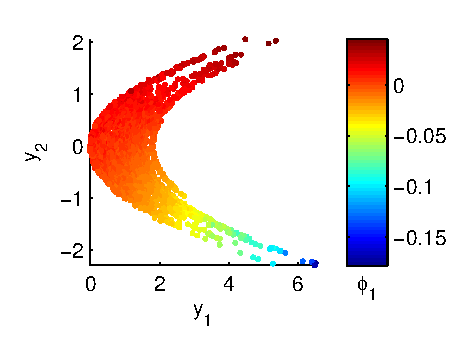
\includegraphics[width=\textwidth]{data_nonlinear_NIV_dt2_kernel1} \\ $\delta t$ is too large};

\draw[->, red] (1.15, 1.7) -- (1.15,1.45);
\draw[->, red] (1.85, -3.35) -- (1.6,-3.35);

\end{tikzpicture}

\end{frame}

\begin{frame}{Reduction of Nonlinear Data}

\begin{tikzpicture}

\node(a){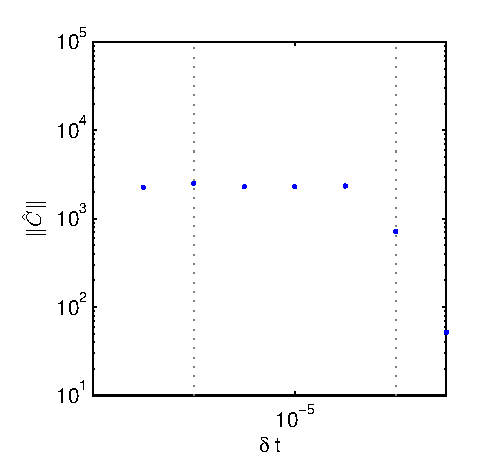
\includegraphics[width=0.3\textwidth]{C_dt_nonlinear}};
\node[below=0cm of a](b){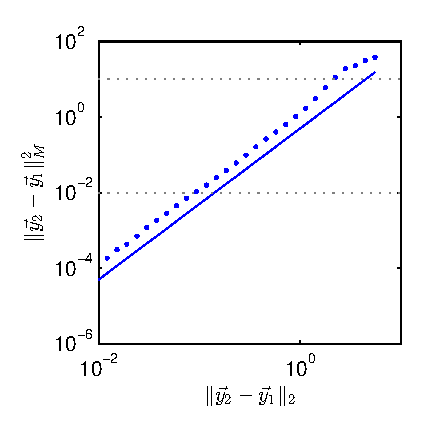
\includegraphics[width=0.3\textwidth]{dist_dy_nonlinear}};

\node[below right=-3cm and 1cm of a, align=center, text width=0.5\textwidth](c){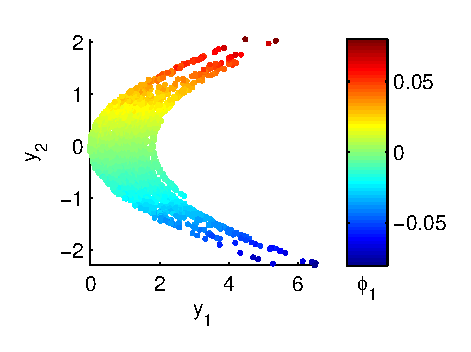
\includegraphics[width=\textwidth]{data_nonlinear_NIV_dt1_kernel2} \\  $\sigma_{kernel}$ is too large};

\draw[->, red] (-0.35, 1.7) -- (-0.35,1.45);
\draw[->, red] (1.85, -2.4) -- (1.6,-2.4);

\end{tikzpicture}

\end{frame}

\section{Conclusions}

\begin{frame}{Conclusions}


\end{frame}

\end{document}

